\documentclass[14pt,a4paper]{extarticle}
\usepackage[english]{babel}
\usepackage[T1]{fontenc}%
\usepackage[utf8]{inputenc}%
\usepackage{lmodern}%
\usepackage{textcomp}%
\usepackage{lastpage}%
\usepackage{geometry}%
\geometry{margin=0.7in}%
\usepackage{amsmath}%
\usepackage{tikz}%
\usepackage{pgfplots}%
\pgfplotsset{compat=newest}%
\usepackage{graphicx}%
\usepackage{fancyhdr}%
\usepackage[%  
    colorlinks=true,
    pdfborder={0 0 0},
    linkcolor=blue
]{hyperref}%
\usepackage{csquotes}%
\usepackage{ragged2e}%
\usepackage{epigraph}%
\usepackage{setspace}%
\setstretch{1}%
\setlength\epigraphwidth{.5\textwidth}
\setlength\epigraphrule{0pt}
\usepackage{wrapfig}
%
\title{Cybernetics Interfaces and Networks}%
\author{Lorenzo Moriondo \\ \href{mailto:tunedconsulting@gmail.com}{tunedconsulting@gmail.com} \\ \href{https://pramantha.net}{Pramantha Ltd}}%
\date{\today}%
\fancypagestyle{header}{%
\renewcommand{\headrulewidth}{0pt}%
\renewcommand{\footrulewidth}{0pt}%
\fancyhead{%
}%
\fancyfoot{%
}%
\fancyhead[L]{%
Review of Techniques%
}%
\fancyhead[R]{%
Page \thepage\ of \pageref{LastPage}%
}%
}%
%
\begin{document}%

\begin{titlepage}
	\begin{center}
    	\vspace*{1cm}
        \Huge
        \textbf{Cybernetics Interfaces and Networks}%

        \vspace{0.5cm}
        \LARGE{intuitions as a toolbox}
            
        \vspace{1.5cm}

        \normalsize{Lorenzo Moriondo \\ \href{mailto:tunedconsulting@gmail.com}{tunedconsulting@gmail.com} \\ \href{https://pramantha.net}{Pramantha Ltd}}
        \vfill
        \textbf{Abstract}
	\end{center}   
    \vspace{3mm}

	Human activities are progressively defined by interactions with products that embed increasingly higher levels of immaterial component (software, patents, design principles and patterns). After presenting the continuity between seminal concepts in Cybernetics, Information Theory, Network Analysis, AI practices on one side and cognitive behaviour by leveraging a minimalist approach to cybernetic systems based on the concept of capacity of network; the text tries to establish the concept of interface to define logical rule-based automata that can be considered shareable instances of a self-model approach to consciousness: in first instance, a rule-based descriptive construct for an 'economy of information exchange' between systems (or an 'economy of time'), and in second instance a rule-based framework for approaching the hard problem of consciousness. These are critical waypoints in navigating fast-growing knowledge-intensive landscapes. This review into patterns of growing complexity is concluded with an hypothesis that aims to extend Ashby's definition of machine to include interfaces to represent self-modeling.
\end{titlepage}%

\newpage

\pagestyle{header}%

\epigraph{
After the tool, responding only to his hand; after the machines, covering complex tasks and operations but subject to his will; here he is to delegate automata to take care of managing and thinking in place of himself, on the basis of apparently rational criteria.\\
\vspace{5mm}
[...] access to text is the worst distributed thing in the world.
}{Henri Jean Martin, \textit{History and Power of Writing}, 1988}


\epigraph{
And the reason that such complexity is not usually seen in human artefacts is just that in building these we tend in effect to use programs that are specially chosen to give only behaviour simple enough for us to be able to see that it will achieve the purpose we want.}{Stephen Wolfram, \textit{A new kind of science}, 2002
\\(about the behaviour displayed by Cellular Automata)}



\section*{Acknowledgments}%
\label{sec:acknowledg}%
Thanks to everybody researching in the AI and Cybernetics fields of enquiry and other scientific endeavours, in particular the works mentioned in the referenced material.


\section*{Introduction}%
\label{sec:intro}%
\hspace*{15mm}This is a collection of concepts and background information useful to define how to approach meaning in a highly interconnected world defined by knowledge-intensive media. Some of those are re-elaborations or follow-ups to other researchers' elaboration or historical reconstructions of the genealogy of concepts; the objective is to add necessary layers to understand and build adequate intuitions for the scale of challenges people and teams are facing in their daily lives as users and professionals.
\newline
\hspace*{15mm}This is an attempt to point to a discourse meant to be both about Cybernetics (a minimalist approach to its cognitive tools, see following sections) and digital technologies (generically referenced as "media"). This approach to \textbf{shareable knowledge description} will be defined in more specific terms, the text will try to create a foundation borrowing from Cybernetics, Information Theory, Graphs and contemporary AI and data practices. In the subsequent chapters we will keep building and reviewing the concepts involved into an hopefully relatively solid shareable cognitive artefact, giving a basic vocabulary to start creating a framework to describe current phenomena (one for all, in a very daring flight, coscioussness).
\newline
\hspace*{15mm}This text is not meant to be an essay about or a history of Cybernetics, if the reader even heard about it. There is already plenty of good material about the subject: some references \cite{ASChistoryrefs,EOLSSvallee,UMPLEBYcybUSA,ROSNAYhistcyb}. Cybernetics-based representations/interpretations are at the basis of nowadays science, technology, experiences and research pathways. It is true the term has lost its explanatory drive due to historical circumstances. For a thorough dissertation about the history of cybernetic research please see \cite{DUPUYmechanization}. For a review about some more historical background that has led to this elaboration please see \cite{heims1980john}. Existing \textbf{concepts and novelties} presented in a different light in this text: \textit{hyperconnected cybernetic systems (HCS, as stepping stone for further intuitions)}, \textit{fractal scale} and \textit{cognitive costs} associated with HCS. The developed outcome is a tentative definition for seminal concepts like: capacity, context as shared semantics in particular about
its role in interfaces as evolutionarly accumulating boundaries between systems, feedback as gain in capacity via pre-shared semantics in the shape of functionally compounded contexts in different layers of applications stacks. The text will try to define a frame and working hypothesis for those novelties and possible applications in best practices. Starting points in current research are studies in Networks, Graphs Analysis and Machine Learning as a team activity proper of data teams; some of which are mentioned in the references. As a general reference, this works starts from the ripples of works carried on by Hofstadter and Dennett \cite{hofstadter_gdel_1979} \cite{Hofstadter1981_HOFTMI_2}.
\newline
\hspace*{15mm}Some brief historical mentions: Cybernetics in its most generic meaning is an umbrella term as it encompasses a very wide collection of research in different fields. Currently it is the basis of relevant concepts in biology like "homeostasis" and "autopoiesis" and major research in AI since the 1950s, besides being the stepping stone for what is called System Theory that has provided the fabric for contemporary worldwide networks. The concept has a quite explicative power in philosophical terms, so much that by somebody it had been seen as quasi-metaphysical. It probably seems to most that the Internet just popped up at some point from very brilliant technicians working on computing hardware, in mainstream discourse the Internet is an orphan in philosophical terms. Or at least there is a missing branch in the genealogy and pedagogy of contemporary practitioners and end-users, that is the stream that starts from Cybernetics and evolves in all the bits and branching happening in the years in-between (for example, System Theory or Organisational Cybernetics to name two). Historically there are just some missing pieces in the mainstream philosophical discourse (combined to the lack of philosophical discourse at all). Putting it in evocative terms, there is a missing corridor in the Archive. Curious people may ask, is it possible that the major knowledge transfer technology of our time has no philosophical backwater in the public perception? If there is somebody that cares about, this is the right place. After thirty-plus years of heavy public usage of The Network is probably time to address these points.
\newline
\hspace*{15mm}Starting from the evidence that reality already is and progressively will be more and more reality in digitised worlds, in both ways of the "real" world becoming more and more digitised and vice versa the "digital" overflowing in the real, we try to build up an archive of usable and reusable concepts to try to understand contemporary scenarios. Not only in the superficial way with the objective of understanding simulated reality, online interactions or how cognition adapt to digital world but also in the wider perspective of the human becoming increasingly "synthetic" (for the chemical  and biological interpretation of life becoming synthetic see \cite{benanti2018realt}, this text will only address the abstract component of this process, e.g. the increased “synthetical” nature of knowledge in the shape of accumulating and sharing digital information in digital spaces).
\newline
\hspace*{15mm}The struggle from the dwelling between digital identities and real-world identities is a major effort for at least two generations now, the "cognitive gap" has roots in the noise around this foundational bit of post-postmodern science, basically many major societal transformation from 1978 onward have some component directly relatable to products defined by cybernetic thinking and its elaborations. The sections in the first half are the attempt to define some cornerstones for defining the cognitive experiences in digitised worlds, hope that they will hold scrutiny and be solid enough to support the building of the (digital) Archive. The second half deals with mechanised systems for effective development of thought experiments to facilitate intuitions to be applied as current practices in an hyper-connected realities. 

\section*{On contemporary society}%
\label{sec:contemporary}%

\epigraph{
If you want peace prepare to set yourself free\\
\vspace{5mm}
Si vis pacem para remissionem}{A. Capitini}

\hspace*{15mm}Automation in goods and services production has been and increasingly going to be one of the main variables to define the state of progress of any developed economy. Supply chains everywhere are informed by automation standards and there are already examples of almost-fully automated production arrays that are machine-controlled with minimal eye supervision (main examples are obviously microchip foundries). This fording from the tools to the robot opened interesting scenarios for manufacturing and service delivering thanks to automation of tasks and automated computation.
\newline
\hspace*{15mm}Goods and services produced through these new instruments have now conquered markets and have a part in billions of lives with their shapes, forms, materials but above all with the immaterial and bulky (for somebody cumbersome) knowledge component they embed. Immaterial is just a substitute for digital, as the bulk of immaterial knowledge is nowadays designed, programmed and encoded in digital form. Consequences have arisen from these applications that require analysis and elaboration: how does this immaterial (digital) load matters in individuals and societies? What are the collaterals of consumption of these products and how to mitigate the constant drifting we experience in our knowledge base? A lot has been presented about sociological consequences and story-telling about these artefacts \cite{UMPLEBYcybUSA} without enough attention to the scientific-philosophic genealogy of these products. Searching the space of ontologies that define these products can facilitate specifications not well carried on by contemporary discourses?
\newline
\hspace*{15mm}Recently, promoted by the rise of industrial standards, reclaiming themes already present in the 1960s, a wide discourse started about which ethics and deontology (especially in the field of AI) is necessary to develop the necessary processes of caring to mitigate possible adverse phenomena manifesting at scale (for a sample of criticalities in digitised process see \cite{Pentland2020} for the particular adverse phenomenon called \textit{drift}, as mentioned in reference). By the adoption of products more and more dematerialised (and so by necessity digitised), the delay in cognitive updating defines organisational disequilibria and is maybe the defining point of the increasingly concerning skill gaps among organisations and individuals and other issues arising in social capital? How can we wrap our heads around these new classes of problems? This text proposes some basic definitions and provides a clearly non-exhaustive working hypothesis to define these classes of problems. 


\section*{Living in digital}%
\label{sec:digital}%

\hspace*{15mm}The process that we call human societies is a journey that manifested itself as a demonstrated emancipation from contingency, that is forceful cyclicity of the cosmos. Every human activity is informed by this necessity, from searching for food to crop rotation, up to the primary instinct to escape death, topical expression of contingent event.
\newline
In the general picture, accepting the metaphor of the global tribe, this continuous process, physical and intellective, aimed to emancipation, needs steps into camping and steps into decamping; a nomadic approach to thinking and decision (in different terms: a continuous search for higher ground to fight against the contingent) that enables humanity to inform theories, philosophies and daily practises.
\newline
\hspace*{15mm}Next section will try to explain and to analyse the acceleration in spreading and transmission of progress (knowledge or information embedded in highly immaterial products and its consequences) that took place since the very beginnings of the Information Age and, as a collateral of this, acknowledging the fact that: in a \textit{high capacity network} (like the Internet, by design informed to cybernetic mechanisms) \textit{what defines groups/systems are knowledge-transfer capabilities} (measured in capacity or bandwidth). Attempting to clear some noise in the definition of “system”, the next chapter tries to set up a foundation for what Sloane in \cite{SLOANdarwin} pages 222-223 defines as a \textquote{comparative study of unifying systems} among the different domains and practices of computational sciences. This foundation will base on feedback circuits provided by Cybernetics; it cannot be otherwise as the \textquote{science of feedback}, beside being seminal to digital products, is also, in the word of an evolutionary biologist (\cite{SLOANdarwin} page 223) fundamental to define evolution: \textquote{In technical terms, human evolution has been a feedback process between traits that alters the parameters of multilevel selection and traits that evolve as a result of other alteration.}. Biology, as other sciences, has been growing the impact of empirical computational experiments in the last decades; modern artificial intelligence applications, as hinted later (see "A Note on…" section), are no less than empirical computational experiments in pattern recognition and decision-making. The “empirical” adjective added to the activity of computational experiments as experienced in the 80ties and 90ties is there to underline the decisive addition of humongous datasets and general replicability of these experiments made possible by current software innovations and practices.


\section*{Media to consciousness}
\label{sec:media}%

\hspace*{15mm}The text tries here to provide some basic features for the creation of a bridge to build up an intuition about the relatedness (the main property of predicates, the capability of representing association between concepts) among some foundational concepts that are manifest to the human experience in a digital world. The main pillars used for the build up are:
\begin{itemize}
\item real-word events (phenomena),
\item experience (observation),
\item media (translational communication, in the double sense of porting from language to language, as in the property of a channel that communicate using a common protocol between nodes; and in a geometrical sense of a isometric movement of a construct from a position to another),
\item science (as the result of iteration and composition of the previous ones to be solid enough knowledge to found other knowledge).
\end{itemize}
These generic features in the field have been pinpointed to be the boundaries (constraints) for these other more structured concepts:

\begin{itemize}
\item \textit{system}: the definition of an object of inquiry in terms that allow replicability among experiments, the text starts with systems with feedback, aka cybernetic systems, but most of the content is relevant to any kind,
\item \textit{interface}: the properties and design principles of permeable boundaries within and among systems, 
\item \textit{“scale”}: in terms on multilevel, multilayer, multidimensional analysis possible for a system; the scale the text aims to provide tools for is what is defined as "fractal" scale. Briefly here the scale at which data manifest challenges for state-of-the-art heuristics, for a general idea of this scale see \cite{QuantaGraphs}); also, for an intuition about how percolating this concept is, at the highest level of a technological stack the "fractal" scale manifests as mirroring between organisations and their systems design as defined in \cite{Conway1967HOWDC}.
\end{itemize}

These structured concepts are therefore used to describe some interesting worldly phenomena:

\begin{itemize}
\item \textit{growth} (biological and informational),
\item \textit{connectedness} (the property of having a channel with capacity/bandwidth, and how to represent connected components in systems), 
\item \textit{cognition} (the orchestration of structures for intellectual enquiries and understanding).
\end{itemize}
And finally also a possible framework for the currently ineffable concept of consciousness.
These will result in an attempt to create tools for the leveraging of structures as a reasoning tool and the description of emergence (like in “emergent phenomenon”). The output will be three main compound concepts coming out from this reasoning: hyperconnected cybernetic systems (HCS), fractal scale and cognitive costs associated with HCS. So basically in general: \textit{systems, interfaces and scales}. Let’s expand on those.

\section*{A cybernetic system in simple terms}
\label{sec:cybernetics}

\hspace*{15mm}Let’s try to clean some noise out from the definition of system and in particular cybernetic systems, aka systems with feedback, that are at the very foundation of the ways peers use to communicate and exchange information. What is a system and its reach to other systems? What are its boundaries? What are systems of systems? This is a brief review of concepts that may provide new insights in the mathematical background for networks as graphs.
\newline
\hspace*{15mm}A system is a collection of components that are connected, empirically they manifest to an external observer a gradient of behaviour that goes from very simple to very complex. Let’s try to define a system in terms of a “group” with the purpose of defining the boundaries of a system. The mathematical tool we are going to use is Network Analysis (and later on in particular the linear algebra representation for graph structures), we start from defining the basic characteristics of a cybernetic network by establishing a definition of what to call a “group” that is a collection of connected components, this is a synonym of “system” depending from the context we are using; please remember this assumption that context is king, meaning is a local matter. Depending at which scale we focus the enquiry group and system can be more or less synonyms, what can be a system for a system analyst can be just a group for a system architect and so on, depending at which scale the epistemic ownership is calibrated, e.g. which is the objective of the enquiry.
\newline
The idea of information networks defined as connected components has been explored by scientific literature (one for all the Measure of Integration of Information \cite{TONONIintegrated} and related), this text is trying to leverage graph of connected components to develop a parallel inquiry taking a step back, to branch from classical cybernetics themes like the ones in N. Wiener's \textit{Cybernetics} and W. Ross Ashby \textit{Introduction to Cybernetics} by trying to enrich them with lessons learned from Network Analysis practices. In general the representation presented here is widely applied to different fields of research, as recollected and systematised by \cite{Pearl2010} for the particular and peculiar case of causal graphs (causal graphs are directed loopless graphs). These in the scope of developing explanatory tools for what we witness in present days as knowledge-production processes and their “complexity”. This is obviously an ex-post endeavour, a recollection of the beginning with the eye of the witness of the world-changing consequences of this invaluable theoretical work. These consequences are the products we use in our daily lives, analysing the causal connections that trace from theoretical work to cognitive effects through digitised products is the main method for the building of the digitised archive.
\newline
\hspace*{15mm}There is no mathematical novelty in what is written below, it is just a cleaned out presentation of a cybernetic system in terms of a graph structure. For a modern example that inspired this approach, the use of a graph to represent a cybernetic network in \cite{dijkstra1978fly}; in which memory of a computer is represented as three connected sets of memory addresses.
\newline
\hspace*{15mm}So let’s start: what  is a group? How can we discern boundaries in collections of nodes that may seem uniform? How do we distinguish groups of "things" from other "things"? Is this the same thing or a similar or a connected thing? A common answer is the ontological approach to define groups or classes based on relatively stable characteristics of the particular things in object; the more objective these characteristics are defined and measured according to the experimental/scientific method, the more the group or class can withstand scrutiny and the challenge of describing the phenomenon. This is obviously a relevant challenge as it is the base assumption for trying to spot causal links to build explanations. Let’s try to create a “grouping” procedure that is not based on ontological assumptions but on connectedness.
\newline
\hspace*{15mm}A reminder of the definition of \textit{bandwidth}: \textquote{... the rate of data transfer, bit rate or throughput} \cite{WIKIbandwidth}. The max possible volume of information transferred on a channel for unit of time: i.e. Mb/s (megabit per second), Tb/hour (terabit per hour), etc. It is not the actual speed of the channel but its maximum capacity per unit of time.
\newline
This text uses channel and connection as synonyms for its purposes. Anything intra-something or inter-something is synonym of in-group interactions and out-group interactions, e.g. inter-system connectivity is anything that the system does out-group, intra-system connectivity is anything that the system does in-group among its own components. Let’s start from the assumption that the only defining characteristic to set the boundaries of a group is its level of interconnection (in-group, e.g. between its own components as opposed to out-group, e.g. towards other groups, see \cite{SLOANdarwin} for this concepts as arosed from multilevel selection), this implies that the only measure that defines a group is the bandwidth among its elements. This makes possible to say that components \(x, y, z\)  are in the same group \(A\) because between them there is a determined level of bandwidth \(w\): (goes to new page)

\newpage
\vspace{0.5cm}

\begin{figure}[htbp]
\begin{minipage}[t]{0.45\linewidth}
    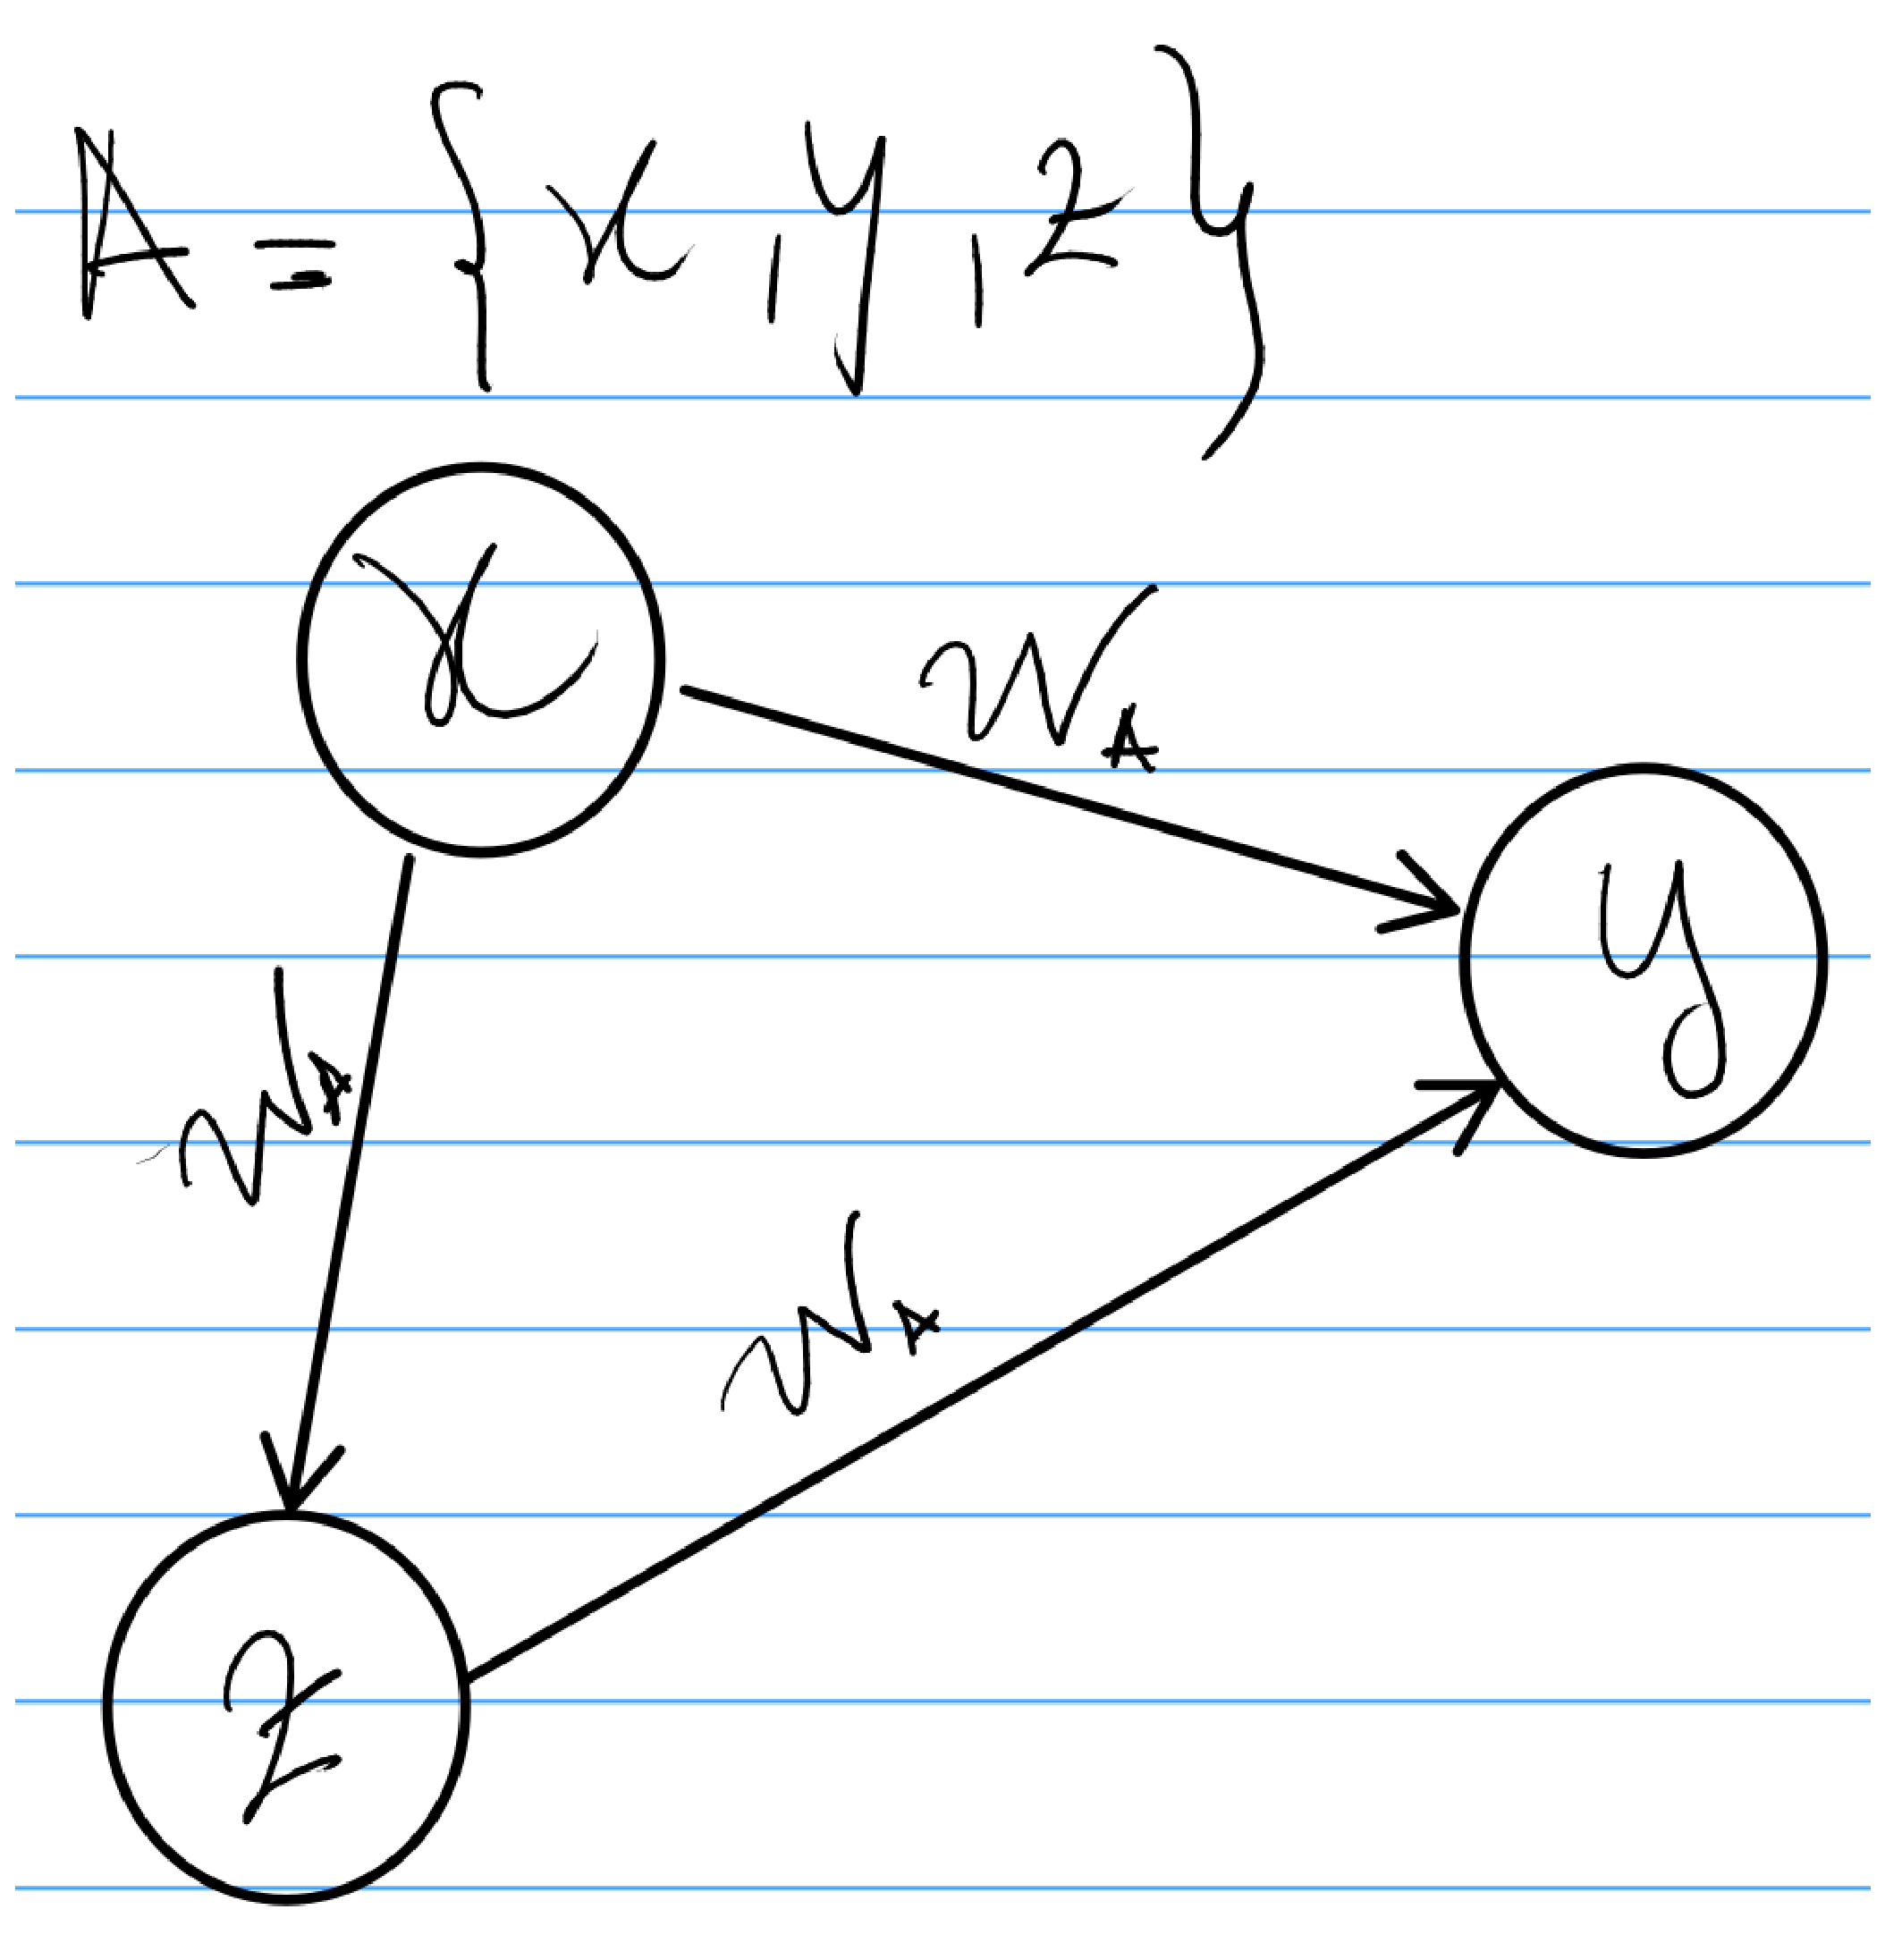
\includegraphics[width=\linewidth]{Fig__1_connected_elements.eps}
	\caption{A system as components\\ connected with channels at the same bandwidth}%
	\label{fig:fig1}
\end{minipage}%
    \hfill%
\begin{minipage}[t]{0.45\linewidth}
    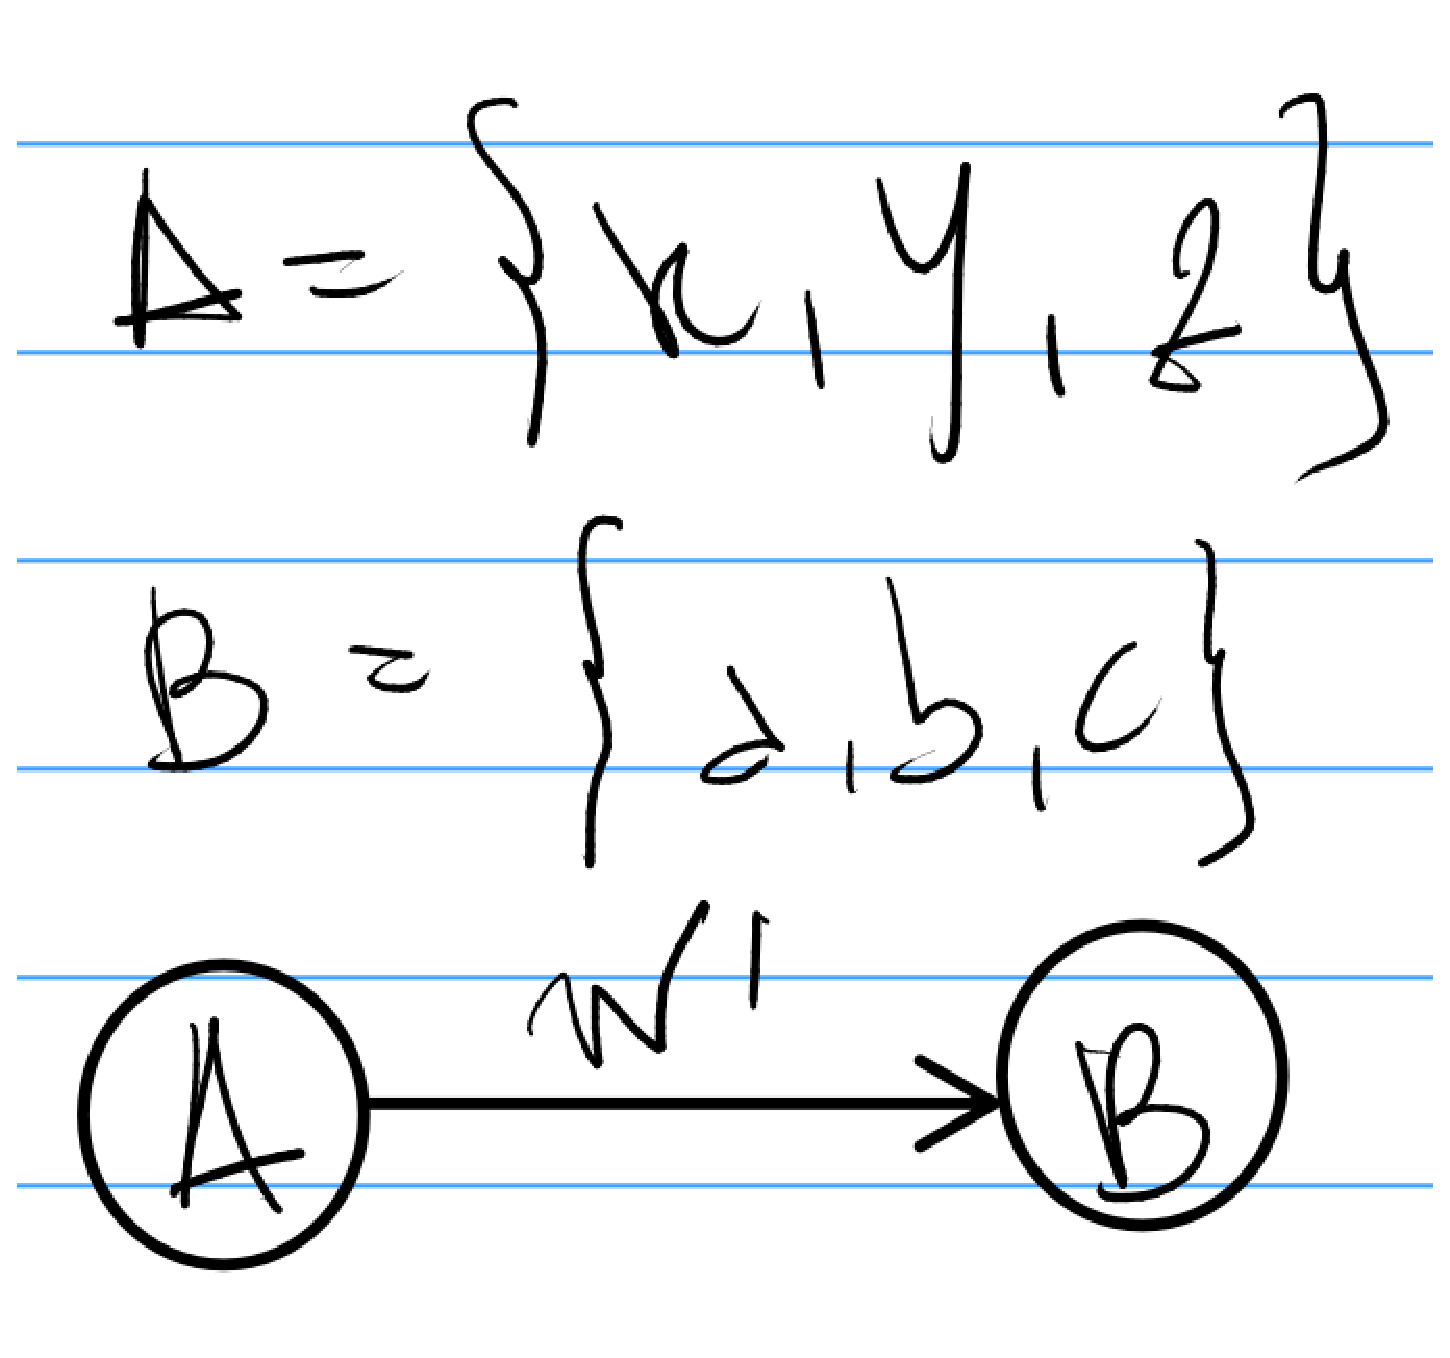
\includegraphics[width=\linewidth]{Fig__2_connected_groups-2.eps}
    \caption{Two different systems for the level of integration chosen}%
    \label{fig:fig2}
\end{minipage} 
\end{figure}

\(A = { x, y, z }\) (Fig.\ref{fig:fig1})
definition of a group, all elements share connection at the same bandwidth \(w\): (Fig.\ref{fig:fig1}) is a directed graph; \(w\) is commonly the weight in a weighted directed graph. Considering the \(x, y, z\) order for columns and rows, the matrix representation of this graph's weights (adjacency matrix) is quite dull:

\[%
A = \begin{pmatrix}%
w_A&w_A&w_A\\%
w_A&w_A&w_A\\%
w_A&w_A&w_A%
\end{pmatrix}%
\]

Assuming that self-connections for each node are working at the same bandwidth as the connections to other nodes in the same system, the adjacency matrix of the group has determinant equal to 0. What if we assume that every single node is not able of self-connection like it could happen in a basic component that is not itself a group or a system?

\[%
A = \begin{pmatrix}%
0&w_A&w_A\\%
w_A&0&w_A\\%
w_A&w_A&0%
\end{pmatrix}%
\]

It may be possible to distinguish basic components (i.e. single nodes or very integrated minimal groups of nodes) from larger systems (i.e. composites of nodes and groups with wider function/scope).
\newline
\hspace*{15mm}The same way in Fig.\ref{fig:fig2}, recursively, it is possible to say that group \(A\) differs from group \(B = \{a, b, c\}\) because between the elements of \(A\) and the elements of \(B\) the bandwidth \(w'\) is different (necessarily lower): \(w_A > w'\) by definition. Any element of one group can have any connection to any element of the other group, any juxtaposed synthetic value of the weights, like the mean of weights from/to elements of the groups, can be used (or either a function, i.e. \(f(w_{xa}, w_{cy})\) if the respective nodes connected are \(x\) to \(a\) and \(c\) to \(y\)).

To sum up the self-similar (fractal) intuition for a system made up of two (or an arbitrary number of) groups as defined as same-capacity nodes, in Fig.\ref{fig:fig3}:

\begin{figure}[htbp]
\begin{minipage}[t]{0.90\linewidth}
    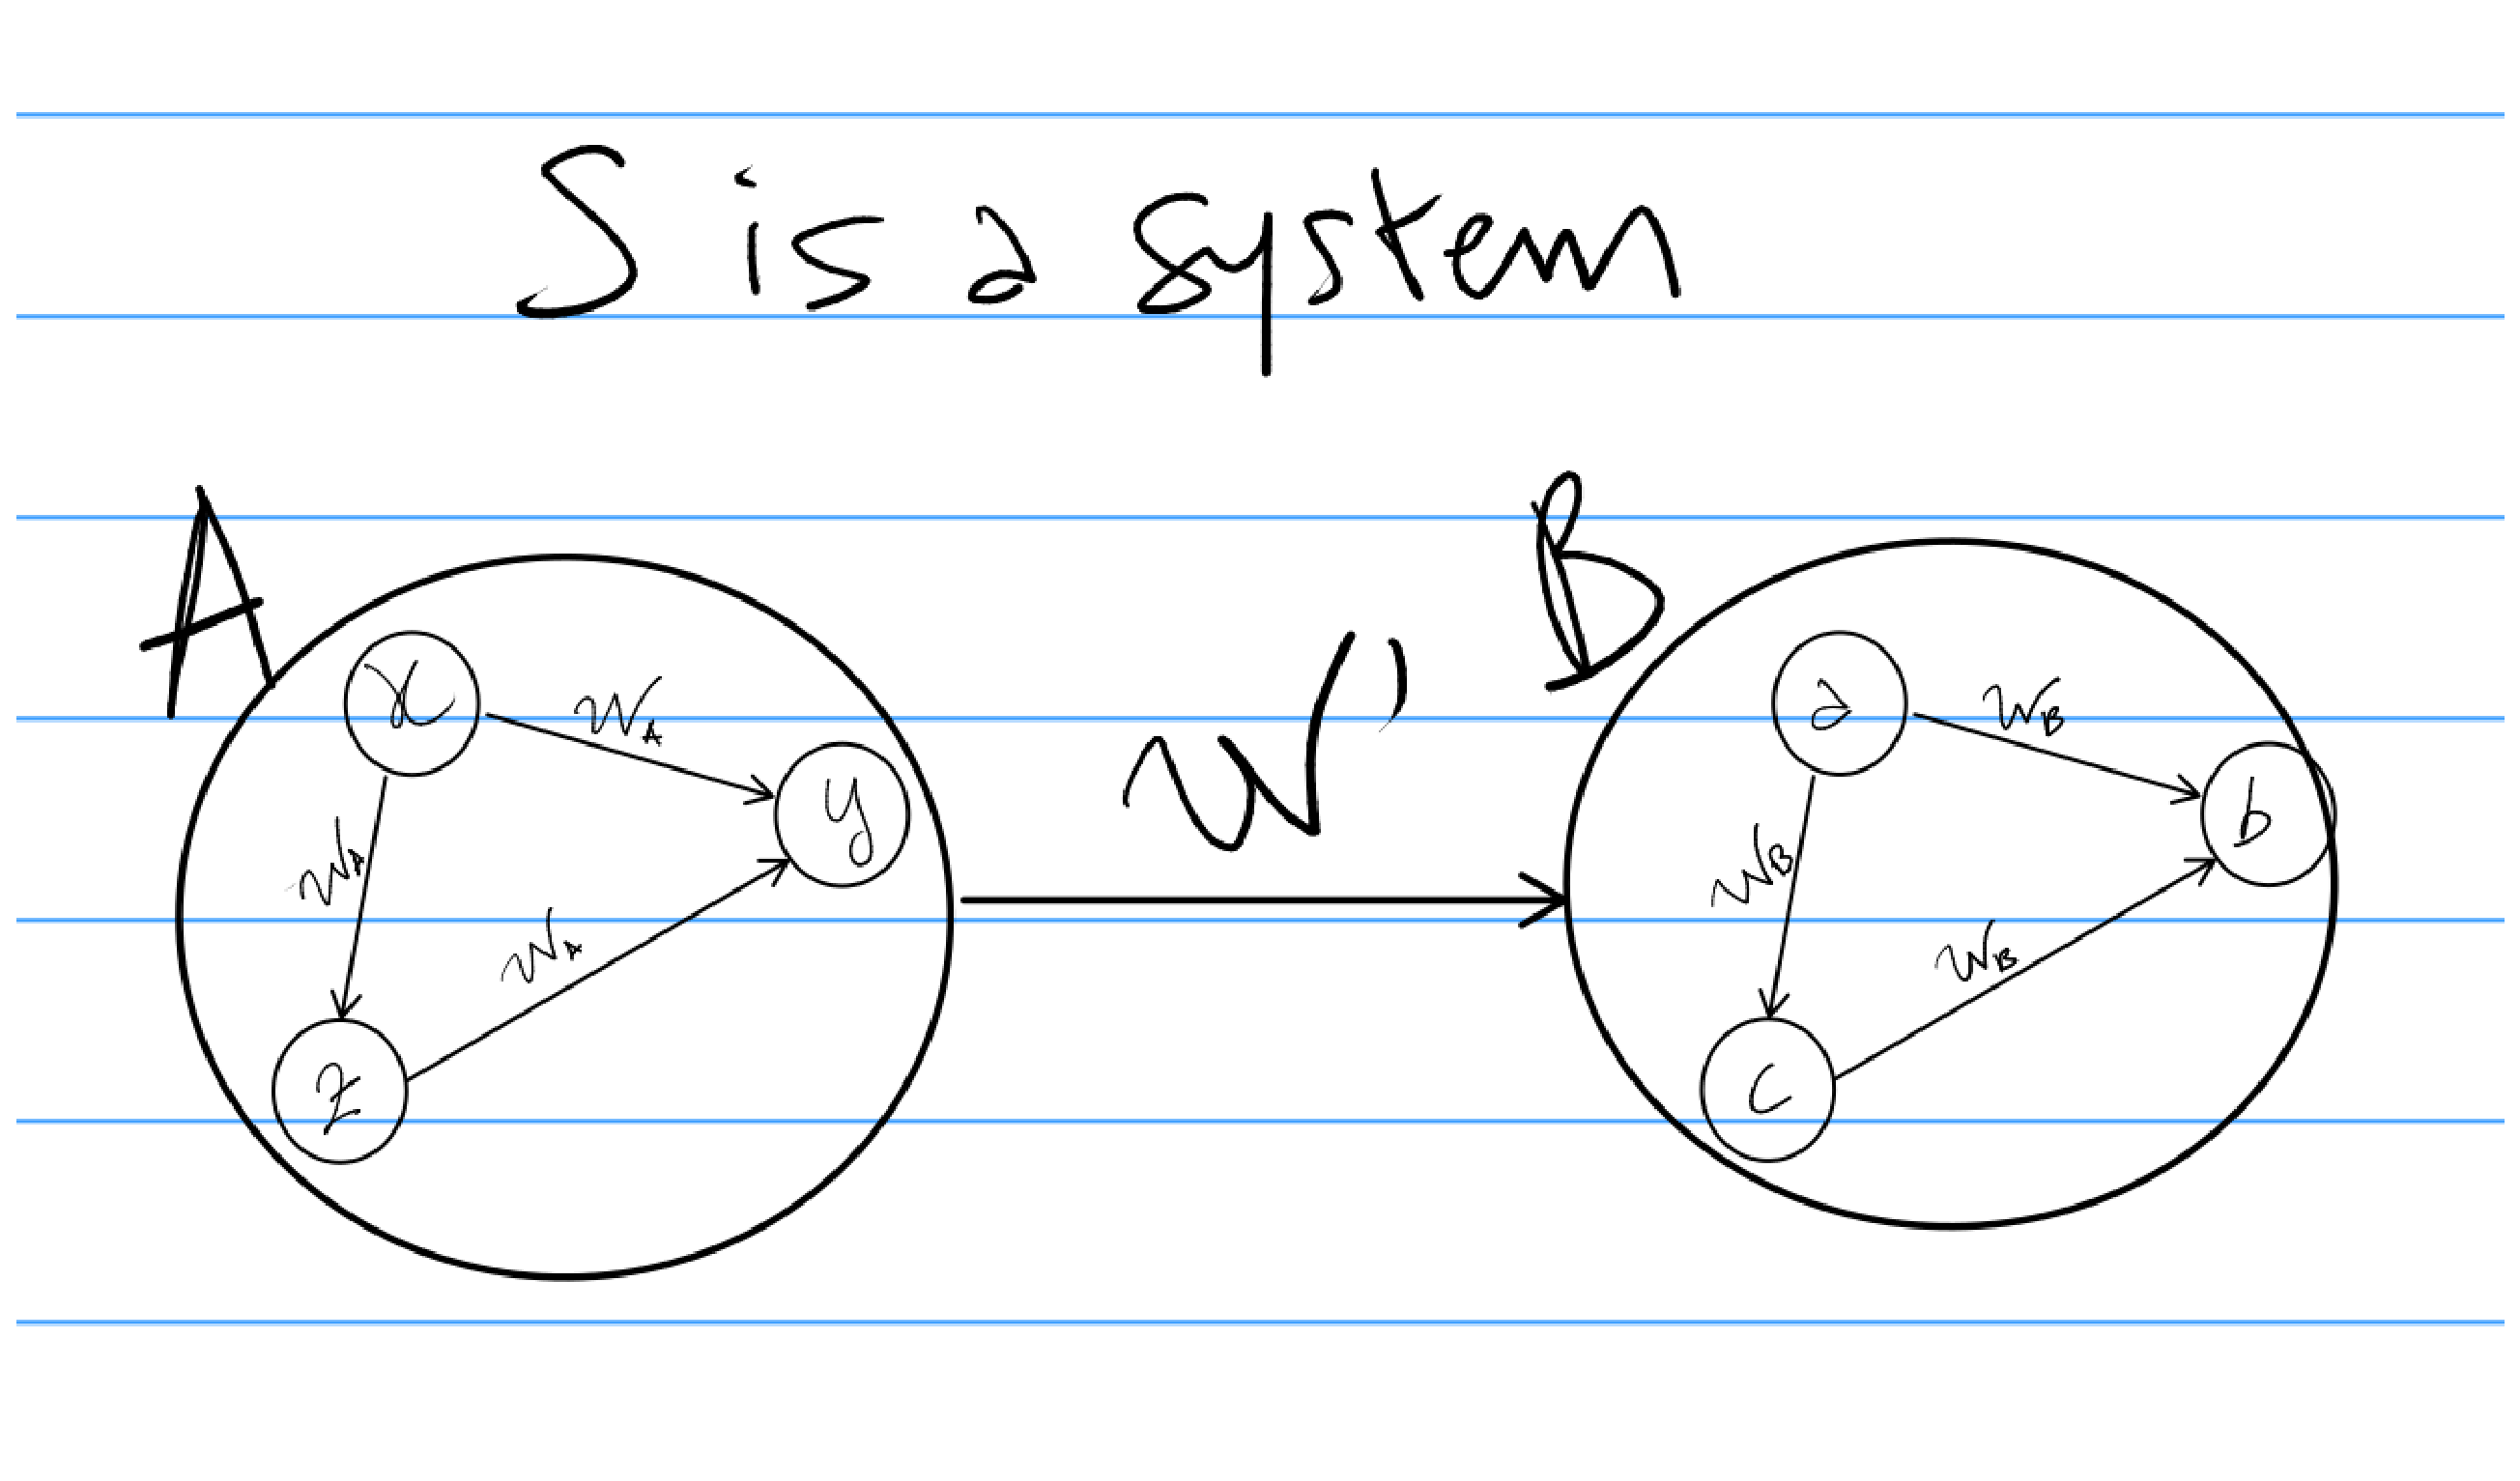
\includegraphics[width=\linewidth]{Fig__3_a_system-2.eps}
	\caption{A system \(S\) between two subsystem \(A\) and \(B\), all defined in terms of capacity}%
	\label{fig:fig3}
\end{minipage}%
\end{figure}

Same assumptions per Fig.\ref{fig:fig2}, by definition it is: \(w_A > w'\)  and  \(w_B > w'\). \(A\) and \(B\) are two separate systems as their shared channel's bandwidth is lower than the channels' bandwidths they use internally. \(S\) is the "global" system (or if you prefer a different word, the context or the experiment) for the observer; for the level of inquiry appropriate for the purpose of the analysis the best scale to limit the boundaries of the observation is probably given by all the components that communicate at a similar level of bandwidth. In the example in the figures, the observation should involve all the components that, like \(A\) and \(B\), are connected at \(w_{ij} \approx w'\). All the components that are connected at much lower or higher bandwidth should be treated as exceptions and considered on specific pathways of inquiry to establish possible relevant interactions with the reference system.
\newline
Recent more formal and practical elaborations on these concepts with an excursus about the evolution of applications based on weight matrices since the 90ties can be found at \cite{KAZUKIselfrefweights}.
\newline
This section is only to review the mapping between graphs and linear representation in preparation for subsequent sections, it is not so trivial though to programmatically search for subgraphs with \(det(A) = 0\) into graphs at scale. It is one of the object of Graph Analysis and related software infrastructures; various techniques have been proposed to spot regularities in graphs, \textit{motifs (or motives)} for example \cite{schreiber2004towards}.


\subsection*{Channels}
\label{subsec:channels}
\hspace*{15mm}The arrows in the diagrams (Fig.\ref{fig:fig1} and subsequent) are what can be called channels (the same as connections for the purpose of this text).
\newline
\hspace*{15mm}\(A\) and \(B\) can themselves be connected components. Any element of \(A\) can have a connection to any other element of \(B\), this establishes a channel (in Shannon’s vocabulary) between the groups: \(w’\) is the mean (for simplicity, or any other synthetic measure for a collection of values) weight of the connections between elements of \(A\) and \(B\) and by definition the average available bandwidth between the groups.
\newline
\hspace*{15mm}\(A\) and \(B\) are then a system \(S\) if exist at least one relevant connection between two of their elements, \(A\) and \(B\) are components of a system.
\newline 
\hspace*{15mm}In this text, groups and components are synonyms depending from the point of view taken; the cybernetician and the engineer will probably prefer "components", either way a component is a group of nodes, and a group is a collection of connected nodes.
\textbf{The thought experiment (model) proposed above defines groups and systems in terms of their capacity (bandwidth)}.
\newline
\hspace*{15mm}Let's take an example that can reach the intuition for most of readers, the speed at which we can think or do self-reflection is perceived to be almost instant, if anybody has an idea he/she can recollect, do logic operation, be predictive about it; all these operations share (approximately for the sake of the inquiry as we have posed it here) the same bandwidth in the infrastructure that is the neural cells network: this is what we call a group or system.
A group (\(A\) or \(B\)) may have many channels to connect to other groups' elements, in the example it can have a channel to another brain system through the way of sight or language, the out-brain communication defined by these channels are evidently at much lower bandwidth than the in-brain channels. So we can say evidently that inter-system connectivity (out-group) takes place at lower bandwidth than intra-system (in-group) connectivity.
This defines the boundaries between groups-systems. The result is two groups \(A\) and \(B\) whose elements can have some connections but by necessity at a lower bandwidth than the bandwidth used for in-group connectivity. So, according to this point of view, different brains can be components in the same system \(S\) but they can also be observed separately thanks to the major difference in bandwidth at which they communicate.


\subsection*{Add Feedback and what you get}
\label{subsec:feedback}
\hspace*{15mm}What makes a system a cybernetic system? This subsection is going to provide the simple system representation presented up to now with an evolutionary leap. The system described above is a simple directed graph described in different layers: the group as description of connected elements and a system as description of connected groups, both connected by channels (this starts to look as a self-similar or fractal structure, the text will analyse this possibility below). 
Starting from the same components as defined: \(A = \{x, y, z\}\) and \(B = \{a, b, c\}\), let’s see what add the cybernetic sauce:

\textbf{Hypothesis:}
\begin{center}
\(x, y, z\) are connected at the same level of bandwidth so to define group \(A\):\\
\(w_{xz} \approx w_{xy} \approx w_{zy} \approx w_A\)\\
Same for \(a, b, c\) defining group \(B\).
\end{center}
\textbf{So that:}
\newline
\begin{center}
With $\rightarrow$ meaning connected and \(i,j\) as index for generic elements of a group:\\
\(A = \{ x, y, z \}\),
for any element of \(A\): \(a_i \rightarrow a_j\) has a capacity of \(w_A\).\\
\(B = \{ a, b, c \}\),
for any element of \(B\): \(b_i \rightarrow b_j\) has a capacity of \(w_B\).\\
\end{center}
\textbf{Definition:}
\newline
\begin{center}
If \(w_A \neq w_B\), by definition \(A\) and \(B\) are different groups or systems if \(w_A - w_B \neq 0\) and this difference is relevant considering the span of the observation.
\end{center}

\hspace*{15mm}Panning the attention of the experiment wider at the slightly larger scale from the group, if we extend this to define a system between groups, by definition: the connectivity between the groups \(A\) and \(B\), taken for simplicity as the mean $\mu$ of the weights of the channels between their elements can be described as:
\[\mu(w_{AB}) < w_A \wedge \mu(w_{AB}) < w_B\]
That is why \(A\) and \(B\) are observed as different groups as their inner connections work at different bandwidth compared to the connection with out-group elements (of the other group); the two groups have by definition a lower bandwidth channel to communicate out-group. They are by construction two different groups. So that again at system scale:
\begin{center}
\(S = \{ A, B \}\) with bandwidth \(w_{AB} \approx w_S\)\\
\(w_S < w_B\)  and  \(w_S < w_A\)
\end{center}

\hspace*{15mm}System \(S\) is made up of the interactions of two groups \(A\) and \(B\) exchanging information via one or more connections among their elements, \textit{if any of this connection is a feedback circuit then we have a cybernetic system}; e.g. a system that is observed as the interaction between an agent and its surroundings or without any pre-conception two systems that interact in a feedback loop.
\newline 
\hspace*{15mm}The two groups by themselves are closed systems, if they have out-group connections between them they are a wider closed system. If we assume that they potentially may develop connections with any other system, they are an open system; again, if any of those connections is a feedback circuit, they are a cybernetic system.
\newline 
\hspace*{15mm} It is straightforward to understand the difference between system without feedback and systems with feedback by representing the former as Direct Acyclic Graph and the latter as a graph with cycles.

\vspace{0.5cm}

\begin{figure}[htbp]
\begin{minipage}[t]{0.90\linewidth}
    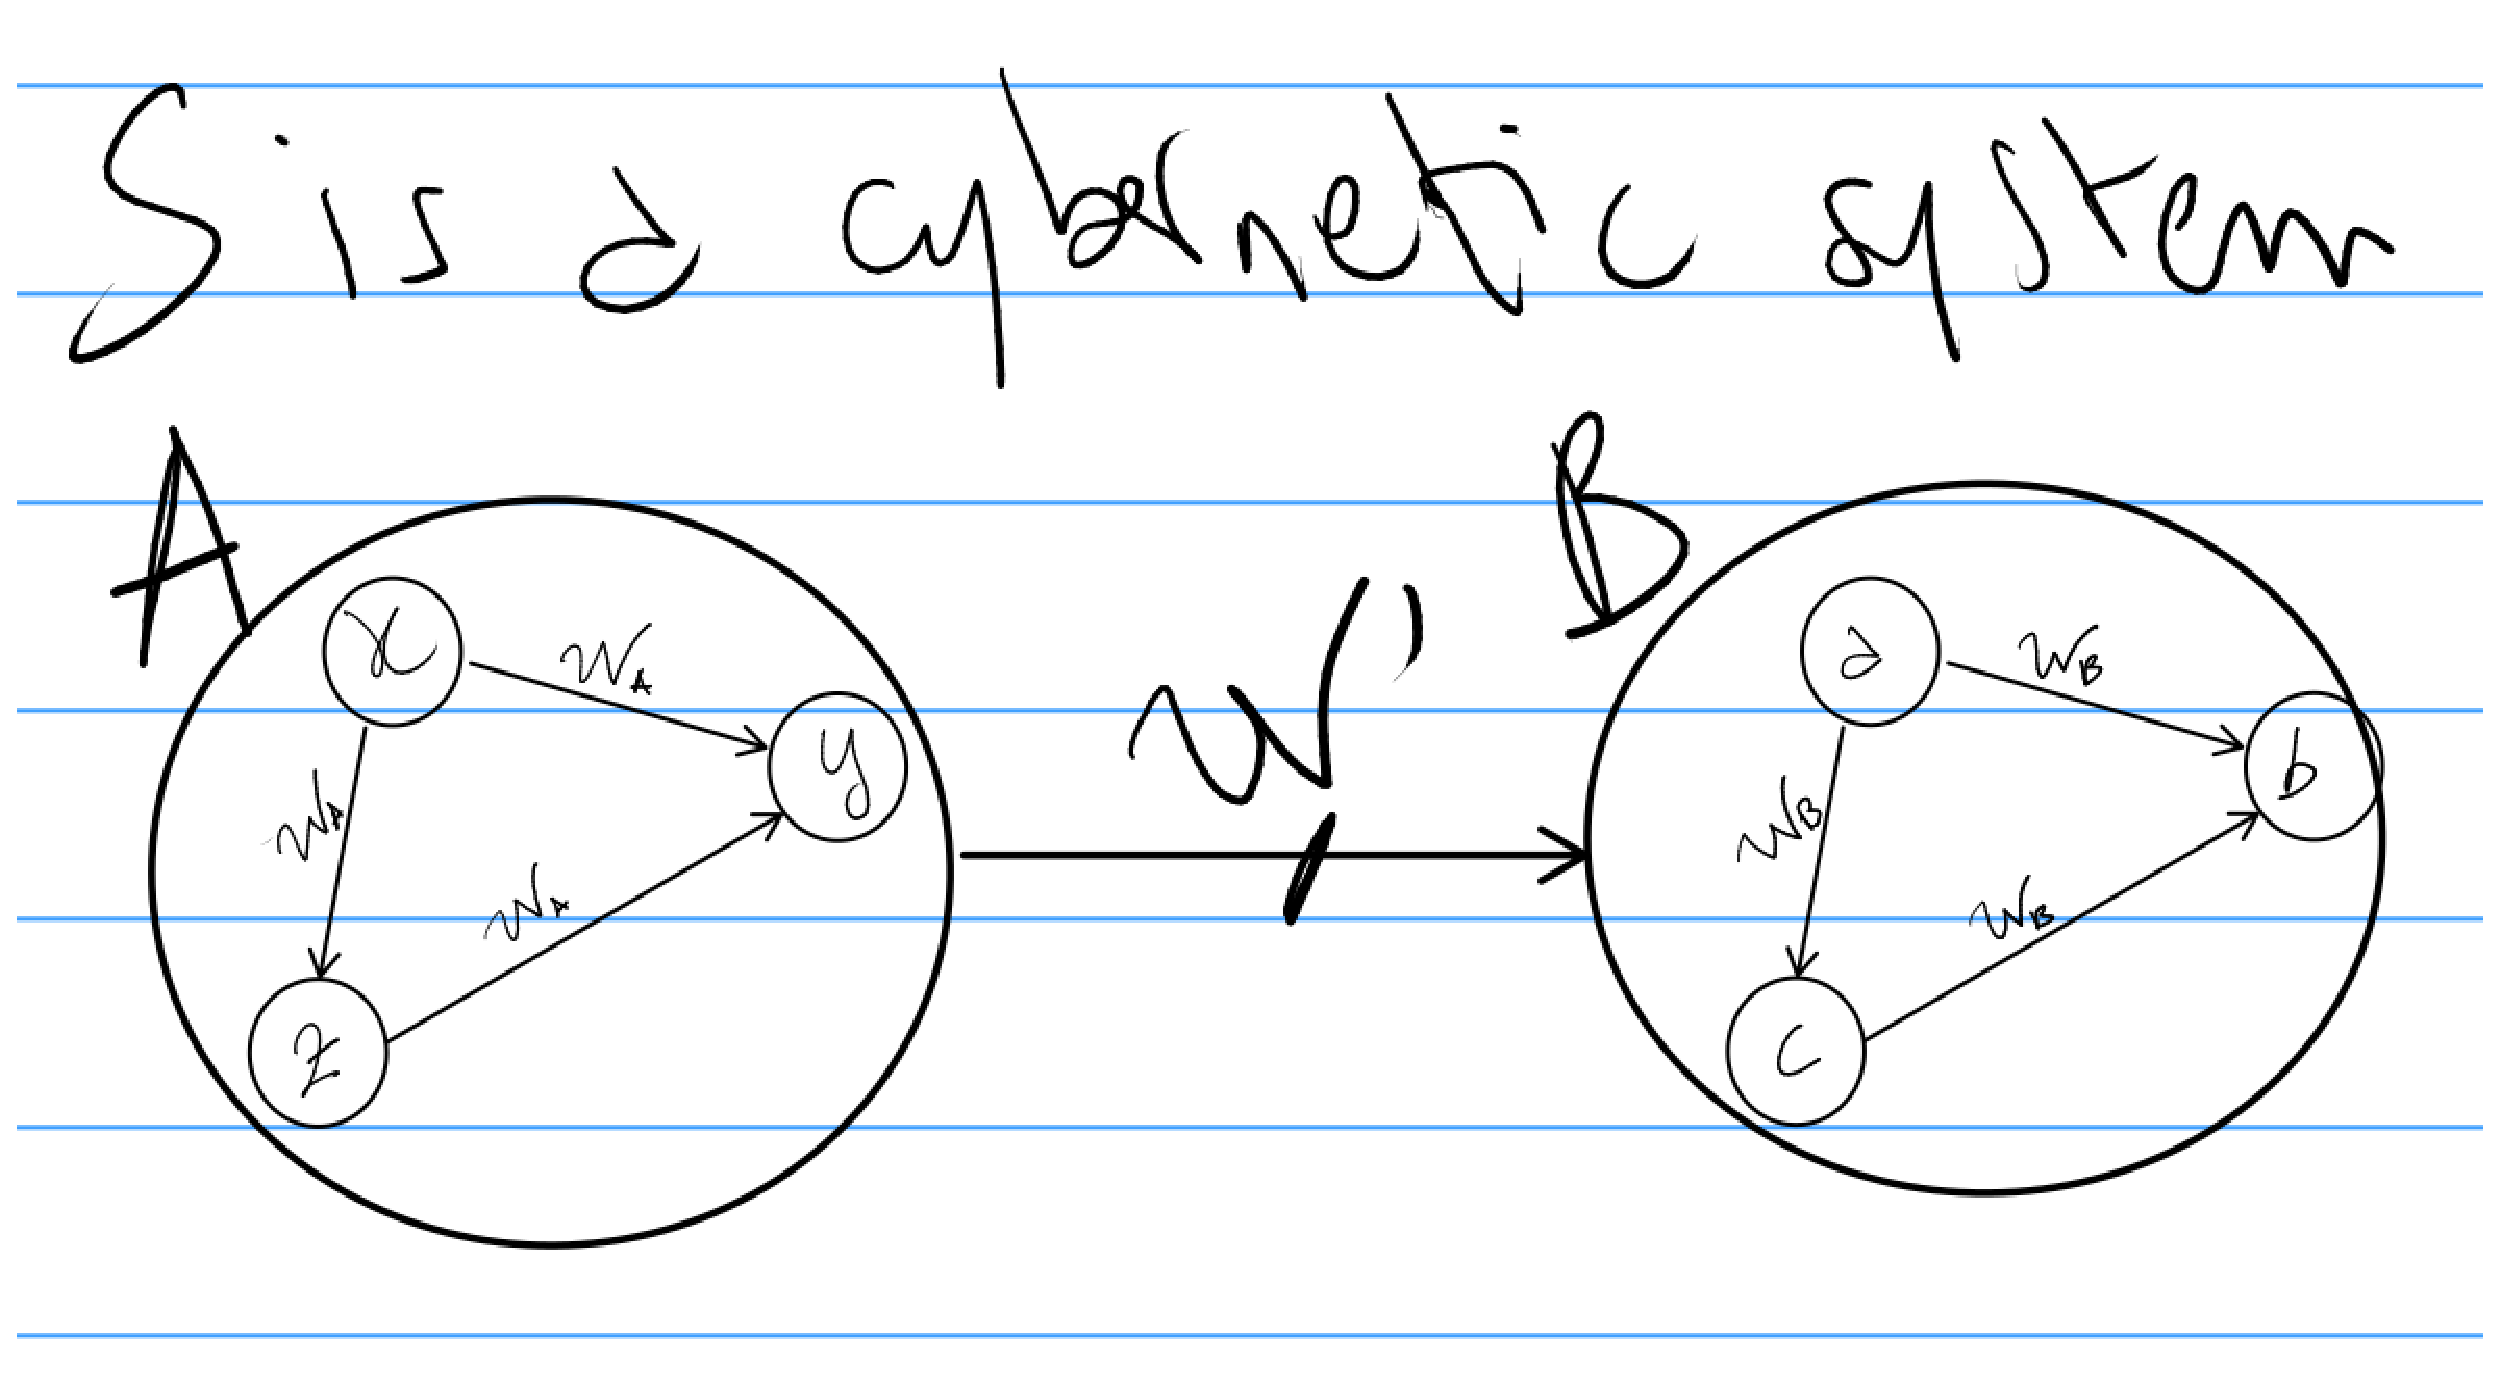
\includegraphics[width=\linewidth]{Fig__4_cybernetic_systems.eps}
	\caption{A cybernetic system \(S\) is a system with feedback, the presence of a feedback channel is drawn as an arrow with a slash \(/\) in the middle.}%
	\label{fig:fig4}
\end{minipage}%
\end{figure}

\hspace*{15mm}This text leaves to other articles and software experiments the linear representation of these networks in terms of adjacency matrices of nodes in the network, in particular the importance of capacity \cite{QuantaFlow}. Trying to make a parallel to current industrial applications: layers in a Deep Neural Network system are the same group as they share the same capacity/bandwidth compared to upstream or downstream layers, but also they are groups themselves if analysed in their single contribution to the stack. Feedback happens between these layers in the shape of backpropagation. Also, and here kicks-in the "fractal" representation, in the context of a Deep Learning Network for example, the model in its entirety as computed from the DLN is a group compared to other subsystems in the same data pipeline.
\newline
\hspace*{15mm}This is a generative (from basic syntactical elements to groups to systems) definition of “groups-systems” for which a group is defined according to the difference in bandwidth between:
\begin{itemize}
\item its in-group elements
\item and the out-group ones,
\end{itemize} 
\textit{a group is a collection of elements that share the same level of bandwidth in spite of any other observable characteristics}.
This is a shift from the ontological perspective (used in both philosophy and software design) for which elements of a group share some observable characteristics or traits, the main problem with that approach is that it can never be exhaustive in listing the characteristics or their modalities as any other list is. These definitions have the advantage of being self-similar and potentially more easily usable for functional and structural analysis. The other relevant question is: does feedback provides gains in capacity? This text tries to reconcile later the importance of feedback as one of the possible ways of "shared memory" between nodes in the same connection and how this "memory" can be part of the information exchange reducing the capacity of the connection, or rather "outsourced" to a in-between standing interface so to have increased capacity. Interface-less and context-less feedback, like backpropagation for example, is exchanged "cost-free" inside the same system operated in the boundaries of the deep stack where the propagation happens; or rather in other occurrences, like HTTP-based Web Interfaces (Web APIs) require instead headers (a context) in every message with or without sharing an HTTP session (another context) over an TCP/IP connection (that establish again its own context). Compatible contexts are defined as composition at every level of the ISO-OSI stack. 
Do interface retain semantics during its evolutionary grow while data exchange happens? Some kind of "intelligent" pattern-matching becomes embedded in interfaces as they iteratively grow?

\subsection*{Experiments and data science}
\label{subsec:experiments}
\hspace*{15mm}This description based on graphs and linear models is a possibly useful representation of the basic tools used for experimental modelling. Software experiments can be defined based on modelled networks and different disciplines take advantage of widely available computation to make use of software experiments at scale for their own objects of enquiry. One particular way of making use of networks is Artificial Neural Networks for which a dedicated subsection is present below.
\newline
A brief mention to define a minimal pathway to experiment designing in the frame of the description defined by this section, that is the abstract model of cybernetic networks based on capacity. The major phases to define a computational experiment in data-centric \cite{Andrewng} terms, that is in the common empirical practice the process of extracting meaning or predictional capabilities from existing dataset, are abstracted as:
\begin{itemize}
\item 1. prepare a proper integration of homogeneous data in a consistent dataset at a wide scale;
\item 2. collect structured domain expertise in the form of programs;
\item 3. run iterations over the software as defined.
\end{itemize}
Considering the frame of inquiry as proposed by this section, major endeavour in executing phase 2. is the process of embedding domain expertise into defining the fittest possible property to be used as index of capacity; in this scenario the most difficult task would be to synthesise the collection of properties for each node in the dataset into a quantitative index that could asymptotically represent a global index of capacity in the context of the dataset. Note: other approaches like Causal Inference \cite{pearl2009causality} require the structured domain expertise to be collected at step 1., also what it is here called capacity is defined in terms of mechanisms as in Structural Equations Models).
\newline
Some basic examples of basic indices of capacity to be applied to networks in different fields of enquiry are: number of common words, or any more or less sophisticated similarity index, between documents in the same collection; throughput of electricity among nodes of a power network; throughput of hormones to receptors; throughput of semi-worked materials along a processing line. All these systems with their own specification of capacity can be also expressed in terms of capacity of information between nodes by designing the right setup for the objectives of the experiment (for example in terms of weights or probability frequencies). This is the very arduous task of \textit{translating domain knowledge into programs, that is itself a very relevant example of a system described by information exchange} \cite{nguyen2008global}. Deep Learning models (a deep stack of ANN) makes this translation automated under researchers' supervision and easily shareable as any other file. There are relevant efforts into making this translation transparent, ethically aware and in the end explainable \cite{enwiki:1083004803}. The outcome from these efforts is the very core needed to create effective machine intelligence.


\subsection*{A note on Artificial Intelligence}
\label{sec:ai}

\hspace*{15mm}Artificial Neural Networks are cybernetic systems, graphs connected by weighted links that undergo feedback (backpropagation) inside larger software architectures.
\newline
\hspace*{15mm}The current most successful (or popular) mathematical representation used in automated pattern recognition and decision-making found origins in the connectionist approach \cite{PlatoConnectionism} and found one of its realisations in Neural Networks Architectures. These computational structures are layers of connected graphs that inherit weights among different layers of deep architectures, each layer is a high-dimensional graph that maps from input matrices to output matrices that are eventually reconciled into value by lower-dimensional layers and activation functions.
\newline
\hspace*{15mm}In the past thirty years researchers have criticised the connectionist point of view putting their efforts in the field of the symbolic approach \cite{WIKIsymbolic,SUNsymconn} but have now seen their theories and applications shaded by the great success of non-symbolic solutions (this text calls them structural of structural-first) based on contemporary Artificial Neural Networks architectures. On another side other researchers with a background in Cybernetics have tried to reconcile the structural approach of Information Theory with a semantic layer that they recognise as necessary \cite{leydesdorff2021evolutionary}. The efforts put on the symbolic and semantic layers seem to have some characteristics in common.
\newline
From the structural-first point of view of ANNs, semantics- or symbolic-heavy tools are needed to be applied to preparatory work and experiment design practices so to allow the ANN structure to provide the fundamental layer for automated pattern recognition and decision-making (phase 1. in the list above), e.g. there is indeed an incredible load of semantic and symbolic knowledge to be applied in the definition of the scope (knowledge needed to design an AI system nowadays goes from software to scientific knowledge to ethics) and preparation of the context for the computational experiment (what it is called in practice data engineering and data preparation with all their phases implied in the work of data science practice). The computational layer itself, in the example taken the Deep Learning Architecture, needs to be “semantic-free” (roughly in the sense for which Chomsky’s syntactic structures does not consider semantics: “I think we are forced to conclude that grammar is autonomous and independent of meaning” \cite{chomsky2015syntactic}) to demonstrate themselves shareable replicable and industrially successful (a focused effort on this particular characteristics has been carried on by "Transfer Learning").
\newline
Symbolic systems have provided some demonstration of success, just an example \cite{SUNsymconn}, but at current state they failed in generalisation, as they are by necessity strictly bound to the knowledge of the researching practices that designed and implemented them; for these systems it is possible to demonstrate success but it is impossible to quantify the extension of their biases. This implies unlimited level of risk, putting it in terms dear to cybersecurity experts: symbolic systems may be fit to the their designed purpose but their threat profile is not quantifiable as result of innumerable possible bias in the designers-defined symbolic or semantic representations, and this denies any possibility of risk analysis. On the contrary it is possible to quantify the threat profile for a structural-first implementation (as a Deep Neural Network), as the major threats will by necessity arise from the scientific and preparatory work done on the data to be fed to the computation (data quality with its own statistical indices), while the computational experiment itself can be “easily” measured in terms of technical threats (bugs, flaws in libraries’ security, flaws in the design of the network). So, from a data pipeline security perspective, a computational layer that embeds symbolic or semantic data in its data and computational structures presents by design a much higher probability of manifesting problematic behaviour if compared to a structural-first implementation. The main driver of risk minimisation is again the work done at phase 1. in the list above. 
\newline
So according to this logic, semantic and symbolic knowledge must take part in the definition of what the shape and the rationale for the inputs are and which scope the algorithm should have, while it should leave the computational architecture to semantic-free structures (like, in the example, Artificial Neural Networks). Symbolic and semantic systems are successful at different levels in a variety of ecosystems obviously, but by design their capabilities will be inextricably dependant to a-priori knowledge that is usually protected behind opaque walls or proprietary systems while for a structural-first experiment the computational phase is the one that is easily shared and contributed to the public; for symbolic system may be a problem if the objective is to provide biases-free operations for every step of the pattern recognition and decision-making data pipeline. Structural-first computations provide major benefits as the ones listed above (biases control, security and many others tha can be identified by domain specialists) and still leave great possibilities both at the preparation stage in terms of human and philosophical perspective and in the computational stage by leveraging human-in-the-loop techniques. As the computational phase is agnostic to proprietary concern, the industrial protection focuses on data handling (data security) and production (deployment and operations).
\newline
There are indeed now new perspectives that row towards the resolution of the symbolic/structural dichotomy \cite{Cheng2016,honavar1995}. Also new viable computational solutions (Graph Neural Networks and Geometric Deep Learning) may be able to integrate at the structural level what are the mathematical representations of the semantic and the symbolic; in this case symbolic knowledge as intended in the 90ties may take part to the selection mechanism in act for ANN with caution in assessing their grade of transferability to target tasks different to the ones they have been trained on. My considerations above still stand, it is desirable to embed considerations related to human-understable and human-readable concepts to the input preparation and engineering phase so to keep the computation phase and the resulting model successful and robust for the objective defined by research teams. In this perspective the semantic and symbolic content should be “statistically abstracted” at a level for which data defines acceptable semantic/symbolic noise and by consequence minimise potential biases. An example of this approach is Causal Inference \cite{pearl2009causality}, the use of causal diagrams as defined in Structural Equations Models to be embedded in the ML model computation (applications of which are labeled as Causal AI).
\newline
Finally, Explainable AI (for an excursus see \cite{savagebreaking}) is contributing to the meta-analysis about how data and computational structures contribute to the resulting behaviour, it may give new insights about how the integration of symbolic and semantic content into computational structures is taking place and how will develop. In particular, the integration of causal structures in the general functioning of ANN is an example of how well-defined (through causal diagrams) semantic content may improve performance of AI systems. Instead for a critique of what I called structural-first (or data-centric) ANN-based systems see \cite{Pearl2018}.
\newline
\hspace*{15mm}All the growing ecosystems defined by these practices, concepts and consequent phenomena are part of current fast-developing scenarios. In the next chapter we will focus on other concepts that, with the concept of (cybernetic) system, are foundational for the description of these scenarios. The following are mostly historical reconstruction of progress made in the last decades with some follow-ups and intuition pumps.


\subsection*{Some intuition pumps}
\label{subsec:cyb_pumps}
\hspace*{15mm}There is no mathematical novelty in what is presented above, it is just a cleaned out presentation of a (cybernetic) system in terms of a graph structure that allows group representation. This leads to some reasoning about in-group and out-group connectivity, how to cope with lowering/increasing bandwidth, groups can acquire/lose elements? Some intuitions pumps:
\newline
\hspace*{7.5mm}\textbf{Transparent versus opaque boxes}
\newline
So a group-system will be observed as such if, from the observer point of view, two or more components are measured to be exchanging information at a given bandwidth (transparent box) or if it is measured to have out-group communications at a given bandwidth (opaque box, e.g. what was a blackbox but thanks to a capacity-based analysis we managed to peak in its inner working mechanisms).
\newline
\hspace*{7.5mm}\textbf{“entangled groups”}
\newline
Can a “resonance” between groups that works at the same bandwidth be assumed? Resonance in the sense that groups working at the same bandwidth may evolve comparable behaviour in feedback circuits. So that two groups-classes-systems can appear to be behaving similarly to an external observer or manifest as seemingly entangled. Hypothesising that working at the same bandwidth can manifest into a similar or identical behaviour even in absence of observable direct communication or previous exchange of information: evolutionary mechanisms can develop the same solutions to the same problem, or a set of similar problems, if in presence of conditions that require comparable fitness. According to this point of view, apt to analyse particular systems like networks that share digital information, mechanisms of feedback could be defined, described or observed and reported in terms of bandwidth only.
\newline
\hspace*{7.5mm}\textbf{A Darwinian intuition}
\newline
Once we have a definition of a group it is possible to spin-off very interesting questions, for example biologists may find it interesting to ask what happens if a group behaves as an adaptive unit?
\newline
\hspace*{7.5mm}\textbf{A quantum intuition}
\newline
As far as it goes my hobbyist-level knowledge of Physics, interpreting what we called capacity as positive or negative probability and assigning to the weights quantities expressed as complex numbers yield a system with the properties of quantum mechanics \cite{Aaronson10.5555/2487754}. E.g. if the system in the diagrams (graphs) above is represented as adjacency matrices in which the weights are quantified as complex probabilities, the resulting system would manifest by necessity the behaviour of a quantum system? If this sounds unlikely, read chapter 9 of \cite{Aaronson10.5555/2487754} to elaborate your own answer.
\newline
\hspace*{7.5mm}\textbf{Biological interfaces}
\newline
About interfaces that retain semantics besides and at some point, while continuing facilitating exchange between systems, they start, after having iteratively grow some minimal structural knowledge of the flow as the data passes through systems boundaries, being able to operate pattern-matching. One example of this is the epigenetic mechanism of methylation, where a mechanism interfacing a memory storage and its replication system acquires a critical function after a long iterative process, taking part in selection according to its own mechanisms (its stored context or semantics) as they work alongside the systems being interfaced.
Another example, that can build intuition about the "multis" (multidimensionality, multilayering, etc. see "A bird-eye view" subsection) and how it is necessary a multi-dimensional approach to elaborate a solid point of view, is current understanding about DNA. Functionally and structurally DNA is a storage for genetic information, it is a "memory" that looks not so much like an interface. Let's try to rotate the point of view in this Bloch sphere that is the "fractal scale" by an n-amount of degrees on one of the multiple axis representing all the possible points of view: from a timed perspective DNA itself is an interface, it is a interface between individuals of the same kin belonging to different generations. The older kin can transmit information in the future via DNA structures and the younger kin can look back at the genetic structure of the previous generation. DNA has developed and keep developing a semantic that make its role as an interface very meaningful. Is it possible to say that interfaces that develops their own semantic are "alive" in the way humans intend it while the ones that keeps their structural (more or less probabilistic) behaviour of growth are not? 

\section*{Interface: the birth child of 20th century}
\label{sec:interface}%
\epigraph{
“If I were a Douglas Adams’
fan I would ask myself: what 42 is
in terms of an interface
in the scope of Number Theory?”
Joke by the Author}

\hspace*{15mm}Now that some basic terms about cybernetic systems have been put down, let’s try to add some other concepts and move into the concept of \textbf{interface}. The concept of interface can be understood well by reading the contribution to complex systems in terms of \textit{boundaries} of a system as defined in \cite{cilliers2001boundaries}. Interface is a largely multidimensional (and applied to multiple layers, for an intuition of multilayer systems \cite{Shchurov2015,Grassi2021,Thakare2021,Thakare20212}) concept, possibly the most self-similar (fractal) concept that emerged from scientific research and applied science in the Information Era. This is its most common usage:
\begin{center}
\begin{minipage}[t]{0.75\linewidth}
\textquote{interface (n.) 1874, "a plane surface regarded as the common boundary of two bodies," from inter- + face (n.). Modern use is perhaps a c. 1960 re-coinage; McLuhan used it in the sense "place of interaction between two systems" (1962) and the computer sense "apparatus to connect two devices" is from 1964. As a verb from 1967. Related: Interfaced; interfacing.}, See \cite{ETYMOinterface}
\end{minipage}
\end{center}

These are different domains in which it is applied \cite{VocabInterface}:
\begin{itemize}
\item \textit{noun} (chemistry) a surface forming a common boundary between two things (two objects or liquids or chemical phases)
\item \textit{noun}  (computer science) computer circuit consisting of the hardware and associated circuitry that links one device with another (especially a computer and a hard disk drive or other peripherals) synonyms: port            
\item \textit{noun}  the overlap where two theories or phenomena affect each other or have links with each other “the interface between chemistry and biology”        
\item \textit{noun}  (computer science) a program that controls a display for the user (usually on a computer monitor) and that allows the user to interact with the system
\end{itemize}
In particular, in computer science, “interface” takes on fractal dimensionality by being applied to boundaries between multiple layers (every layer of the software and hardware stack): between devices on the outside of a system, between the different layers of the software stack on the inside of a system. From the top layer, the user interface (4. In the list above), to the depth of the hardware and its abstractions.
\newline
For the software experts: function signatures are interfaces, but also the collection of function signatures belonging to the same package or module are indeed interfaces.
\newline
\hspace*{15mm}In linguistics, modules like phonology, syntax, semantics and pragmatics communicate over interfaces and the handling and learning of a language require mastering these relations \cite{Lanthi2006}. Intuitively, collections of names with a common domain of application are interfaces as they are boundaries between multi-layered concepts and their shareable representations.
\newline
\hspace*{15mm}Let’s try to build some intuition on top of some recent research that involves the concept of interface:

\begin{enumerate}
\item The working hypotheses related to abiogenesis, e.g. the formation and emergence of organic compounds that brought to life-as-humans-know-it on this planet \cite{lingam2021life}
\item The mathematical definition of growing interfaces as presented in Kardar-Parisi-Zhang (KPZ) equation and demonstrated by experiments on growing interfaces of liquid-crystal turbulence \cite{PhysRevLett.56.889,Takeuchi2011}
\item Interfaces in software stacks
\end{enumerate}

\subsection*{1. Membranes and natural interfaces}
\label{subsec:membranes}
\epigraph{
"We often fall into the trap
of thinking of a boundary as
something that separates
one thing from another. We
should rather think of a boundary
as something that constitutes
that which is bounded."
Paul Cilliers, 2001
}

\hspace*{15mm}In the domain of life sciences interfaces take the name of membranes. In particular some research about abiogenesis and the fundamental role of boundaries in the different hypotheses around the emergence of life provide nice examples.
\newline
\hspace*{15mm}Many hypotheses are on the table for the formation of life on this planet, to name a few very generically: metabolism-first, replication-first, co-evolution of RNA and DNA \cite{lingam2021life}. There is one evident common constituent property for all those: boundaries, the formation of \textbf{membranes} (an interface that is evolutionary developed between any developing molecule and the environment), in particular the formation of vesicles in accordance to molecules’ characteristics (necessity of storing genetic information and replicating it) or environmental conditions (underwater hydrothermal vents). Very briefly, pockets of molecules that can sustain themselves through endothermic reactions probably happened to come together to later start Darwinian evolution.
\newline
\hspace*{15mm}Let’s try to unpack how in these hypotheses two types of interfaces, \textit{membranes around these pockets (biological interfaces) and ecological (so called ‘natural’) interfaces} have a decisive role. In one of the abiogenesis hypothesis, membranes seems to had evolved by atomic accretion attached to flattened spherical natural rock formation (underwater volcanic rocks) to form vesicles of non-organic material; this kind of isolation from the external environment allowed the creation or acquisition of more complex internal capabilities that had been since then subject to natural selection.
\newline
The membrane is one of the decisive parts for the working of the hypothesis \cite{lingam2021life} as the initial structural feature since then was able to tweak its own fitness via adapting feedback to the increased or decreased external pressure; without the membrane (the interface) there would have been no regulated way of feeding back between the internal and the external of the vesicle.
\newline
Furthermore on the concept of interface: most of the abiogenesis hypothesis \cite{lingam2021life} consider as decisive the presence of local chemical conditions that facilitated the rise of complex pre-organic and organic compounds. These conditions are the ones present for example in the air-water interface as found in volcanic ponds, where water sublimate in steam and the particular pH gradient allows all sort of chemical experiments to happen (see \cite{lingam2021life} page 135); speaking of the the natural interface between the oceanic water inside and outside the underwater vent: \textquote{A unique feature of the pH gradient observed across hydrothermal vents membranes is that their magnitude and polarity … are both commensurate with with the gradient associated with biological cells. In particular, the novel mechanism (chemiosmosis) underlying the synthesis of ATP in cells .. entails the movement of protons across the membrane, quite reminiscent of water flowing across turbine.}
\newline
\hspace*{15mm}The concept of interface is the best example of what a multidomain concept is. The concept of interface is fit to reach applicability (somebody would call it fitness) to explain complex behaviour in different observational domains; this feature, together with multileveling/multilayering and multidimensionality are the three clues that can highlight fractal invariance, a very useful descriptive tool for the empirical computational observer (for a mathematical representation of this “multis” and their implications see [31]).

\subsection*{2. Growing interfaces of liquid-crystal turbulence}
\label{subsec:crystals}
    
\hspace*{15mm}As membranes can be abstracted as interfaces, also crystals growth leverages this concept successfully. The generalisation for this feature is modelled by Kardar-Parisi-Zhang equation [18a] that mathematically defines how an interface grows on a flat (at atomic level) crystal surface that happens to be hit by a laser of growing intensity. The growth of the boundary is mathematically defined by the equation, the characteristics of the boundary are the one observed in [18b]

\subsection*{3. Software interfaces}
\label{subsec:software}

\hspace*{15mm}It would be too long to give a comprehensive account about how decisive the concept of interface in computer science and software engineering is. Application Programming Interfaces (APIs) have been starring in one of the major lawsuits among tech giants, in which the main point was if APIs are by themselves medium for knowledge transfer or not. Very briefly, if copying the thin layer that connects different software components implies copyright infringement. Are APIs Commons?
APIs in software are the perfect example of a multilevel/multilayer concept as it spans at every level of the tech stack from low level programming to Web APIs. This is quite natural as the computer medium itself is defined on functions calling and recursion. I won’t annoy here the reader with more of this even if I could extensively (see my previous articles).
\newline
\hspace*{15mm}This leads to what APIs/interfaces in general are in cognitive terms? They create standardised comparable meanings between a domain caller, an agnostic callee and a domain responder: the only thing that allows us to reach into a blackbox is an interface for accessing/setting and returning  data to/from the box. Do interfaces define a “meaning delta” to facilitate logical connections between segregated layers/dimensions/domains? Can interfaces be used as languages, as shared pieces to exchange knowledge?


\section*{Scales of challenge}
\label{sec:scales}%

\hspace*{15mm}The concepts of system and interface have been recollected and extended in the previous paragraph. It is missing a spark thought, why are those in need of extension and why some adaptations and maybe new traits are needed. The stimulus to this change is the set of multiple challenges put forward by data at scale both in the research about the micro- than about the macrocosm. Starting from the perspective that we can somehow see unifying features between the observationally opposite micro and macro; calling these features, these “topological” or “geometrical” continuities between phenomena in different domains and different scales as \textbf{fractal scales}. Previously we tried to build an intuition about this concept by putting the boundaries of those scales in the realm of hypergraphs as mathematically challenging representation of cybernetic systems; it is indeed a hint that graphs are simple representations that needs a great amount of computation to be harnessed, the answers they can bring are well guarded by an exploding complexity as the edges grow.
\newline
\hspace*{15mm}Researchers are taking time to generalise graph theory and the starting point are obviously always high-dimensional datasets (see [31]), the point is to try to find invariants between single nodes and groups of nodes (for example to explain phenomena like peer pressure or biological response to viral infections). This is a fractal scale or at least its boundaries as there are already present the characteristics of the fractal in the shape of being multilevel (single and groups) and multidomain applications. Tools and practices built on large datasets (in general “data-driven”) are inherently explorative compared to more synthetic representation like mathematical induction or descriptive representation like statistical indices, obviously mathematics and statistics are foundational to exploratory data analysis and machine learning practices.
\newline
\hspace*{15mm}Another hint of what it is the challenge of fractal scales can be found in \cite{haferkamp2022linear}, fortunately the proof of the conjecture as presented in the paper gives human-scale humans some positive benefit of doubt about the possibility of developing cognitive tools to harness fractal scales. By proving that \textquote{the complexity of quantum circuits generically grows linearly for an exponentially long time}, beside drawing a connection between complexity as computed from random quantum circuits and the volume of wormholes (aka Einstein–Rosen bridge), the paper suggests that up to a certain scale of time (measured with the exponent of complexity for a given number of qubits) complexity grows linearly; there appears to be a (quite high indeed) threshold in the “life” of a wormhole at which complexity holds. Is this a boundary or an interface?
\newline
\hspace*{15mm}All the search space between social graphs up to mature wormholes and down to abiogenesis (and, in another dimension, from the determinant to the Hamiltonian) is the space of fractal scales reasoning with all its interesting knowledge waiting to be harnessed. This requires a well informed process to provide shareable and diverse knowledge to be put at work into structural-first software machines (for an example see the data-centric AI initiative); the with for this kind of processes starts from how the individual shapes the self as a cognitive behaviour. This brings us to the next paragraph.

\section*{A framework for cognitive costs}
\label{sec:costs}%

\hspace*{15mm}After the presentation of these concepts that are meant to be tools in the toolbox, this chapter will try to bring the discourse back in the field of social impact. In the world defined by digital networks every missed opportunity of adaptation (bias, prejudice, dogma, taboos, or just latency and attention deficit) translates into costs accumulation for future necessary adjustments.
\newline
\hspace*{15mm}Individuals/societies/cultures (organisms or complex systems defined on different fractal scales, but inside the same fractal frames, an example of fractal frame in biology is multilevel selection hypothesis \cite{doi:10.1111,10.1086/286046}) accumulating [cognitive, informative, adaptive …] costs in excess find it more and more expensive their fight against contingency and demonstrate additional stress. This text tries to find some basic steps by borrowing some vocabulary from Networks Analysis \cite{BRANDESnetwork} and Feedback circuits (neural systems and electrical circuits are intertwined since the beginning of research in the field, see \cite{heims1980john} chapter 10).
\newline
This model tries to iterate over the transmitter-receiver model in which nodes are both transmitters and feedback broadcasters. It may be needed to develop an extended concept for feedback that implies a receiver that provides feedback to the transmitter but also defines consequential spillovers to other connected nodes (as tried in section "A cybernetic system"); those are not feedback in traditional cybernetics thinking but themselves transmissions that reach other nodes via open channels that themselves trigger feedback. To be very synthetic, \textit{the scenario that opens is made of structures like hyperconnected graphs (hypergraph or tensor) built on the basic representation of a cybernetic network with spillovers as applied to human-defined networks}; let's try to imagine this kind of system applied to cognition in a scenario with abundant information:

\begin{itemize}
\item A. [Hypothesis] “Capacity is fitness. If a node does not make use of capacity, it necessarily accumulates costs”. Is it correct to assume marginally increasing costs at a given ratio (linear, compounded, exponential depending on which network is used as a base model) with the increase of unused available bandwidth?
\item B. [Hypothesis] “A system that uses the full (available) capacity of a network does not accumulate costs”. Is it useful to propose as an ideal reference that the highest available capacity is the reference value of that particular cybernetic system that does not accumulate costs (perfectly adaptable on the available network)?
\item C. Being the main point shareable information, not raw quantity of information, hence relative importance goes to capacity (flow) instead of stock; this puts priority on knowledge transfer capabilities (throughput).
\item D. [No meaning without feedback] In a network, the circuit between a transmitter (a node) and a receiver (another node) is defined as a cybernetic circuit (presence of feedback, direct or indirect between nodes)intermediated by interfaces, otherwise there would be no semantic. This is related to the concept of “meaning” in the context of an algorithm (meaning of an algorithm) in the sense that the meaning is the reason (ratio or effective procedure) of the algorithm. Direct feedback can be interpreted as proximate causality, indirect feedback is usually byproduct or spillover; reconstructing a chain of proximate causes (in an hyperconnected graph representing a system) can manifest ultimate causality. Extreme hypothesis: meaning is accumulated feedback, e.g. meaning can only emerge or be recognised if feedback mechanisms are possible (aka there are working and fit up interfaces between nodes of a system and those are the fittest representations for meaning as built by the interaction of the systems)? 
\item E. [Another look to entropy] By its own definition overhead (context) always lowers capacity (at constant bandwidth). Transmitting, receiving and feedback require capacity.
Any potential or desired balance between stored information and available information (among nodes) implies updating costs. Direct feedback implies very low overhead. Indirect feedback (spillovers) implies higher costs but it can still be justified in terms of efficiency if compounding with other similar effects (byproducts).
\item F. Indirect feedback comes with the necessity of a context; a node can receive indirect feedback (feedback not directly received, i.e. spillovers, or intermediated feedback) but it can make use of it only with information about its original context. Context requires an overhead (ask the “context is king” people \cite{doi:10.1057}). In the case of cognition, context comes usually in the frame of semantic/symbolic content.
\end{itemize}
\hspace*{15mm}Lacking in foundational knowledge in the mechanisms mentioned up to here is evidently relevant in explaining dynamics about the skill gap that is the starting point for the excess of stress and estrangement experienced at personal and social level after the sudden diffusion of digital networks in general public; it is a relevant struggle both on the before and after of the event (singular, according to somebody) that will bring the entire population to be digitally connected.

\subsection*{Working hypothesis: a toolkit for network technology at scale}
\label{subsec:toolkit}

\hspace*{15mm}A working hypothesis on the self, aimed to mend or reduce cognitive gaps, can be defined as \textit{medium-driven approach}. Digital products cannot be anything more than embedders of informative processes that in the upstream generate the immaterial components of the products themselves; those are the seminal concepts and the philosophical terms on top of which the processes are built; to allow the mapping of the self so that to let the potential of expression allowed by current high-capacity networks to be unfold in researching the path of the fractal scale. The anchor points used for the triangulation that allows the calibration of cognitive tools:
\begin{itemize}
\item \textit{epistemic ownership}, that we will try to explain as capability of reading the meaning (of the algorithm, i.e. the presence and complex interactions of feedback). This is an extension of what is generally known as the point of view of the observer; the point of view is never completely objective, to avoid biases it should always be explicit what is the researcher's epistemic ownership and how it was acquired (back to “context is king” \cite{doi:10.1057}). 
\item \textit{complexity}: the \textit{evolutionary dynamics of cybernetic systems as hyperconnected networks} that the scientific discourse allows to approximate reliably in their spatial-temporal dimensions; the dimensions of the fractal scale requires an adjusted framework for causality and emergent behaviour.
One of the objectives of this text is to facilitate an intuition of fractal dimensions (self-similar at fractal scale); the axis of multileveling, multilayering and multidomain can be approximated by cybernetic systems in terms of groups and groups in terms of constituent groups (aka components). 
\end{itemize}

\subsection*{A bird-eye view}
\label{subsec:bird-eye}

\hspace*{15mm}Epistemic ownership and the idea of evolutionary dynamics of systems are examples of the concepts needed by a modular framework to work out invariants of an observed fractal-scale phenomenon; these moduli are functional to the creation of appropriate vocabularies for the reading of meaning related to digital networks. The collection of these vocabularies (aka an ontology) is an archive built on these moduli; each modulus is defined in historical-evolutionary terms (in this particular field of enquiry, archaeology of digital networks) and it relates (better it accumulates in stacks, it stacks) to others through well veiled structures of multilevel causality \cite{ScholarMultilevel} (connections or invariants between different layers of the stack); multilevel, multilayered and multidomain causality at scale manifest fractal causality. Fractal causality can be researched with structural-first experiments, that inform in feedback loops the vocabularies. \textit{The most (and probably only) relevant source of feedback to inform the symbolic layer is functional analysis of the network/experiment as engineered from abundant data (ideally at fractal scale)}. This is justified by the fact that every object of inquiry is the product of an evolutionary process, the objective of functional analysis is the reverse engineering of the mechanisms that generated the traits that fulfilled the fitness required by the selection. The symbolic is the layer at which teams receive and share feedback and tweak the experiment (may it be considered a particular type/group for a node: observer node). For an example of how experiment design, ethics and other “symbolic-intensive” domains provide the base for the experiment and receive feedback from experimental iterations see \cite{Andrewng} and all the organisational and theoretical work done on data-centric AI.
\newline
\hspace*{15mm}What fractal scale means in the context of the reasoning about the multiplicity of digital worlds, can it be a useful abstraction as a "unifying system"? \textquote{It is important to remember that unifying systems exist throughout nature. The same theory that explains human groups as adaptive units also explains social insects colonies, individual organisms, and even the origin of life itself as unified groups of interacting molecules that evolved by group-level selection.} \cite{SLOANdarwin}. Group-level selection as intended here belongs to a set of concepts that this text is trying to specify to be fractal concepts or fractal invariants; a kind of concepts that hold explicative power (carriers of meaning) in a multilevel, multidimensional and multidomain context. A fractal scale is then a wide range of discursive contexts unified by functional analysis, it possibly maximises the reach in the three dimensions relevant for explicability: multileveling/multilayering, multidimensionality and multidomain. All these “multis” are the axis of what this text tries to define as fractal scale (the Bloch sphere of possible points of view), one of its mathematical description is the hypergraph (for a generic overview see \cite{QuantaGraphs}) whose nodes are connected by feedback.
\newline
What are the challenges posed by fractal scale in a scenario in which data is abundant?
\newline
\hspace*{15mm}\textit{Causality} in non-linearity is the main challenge in a network-threaded scenario as in any other scope; patterns can be “recognised” in high volumes of data (see [31] to know which volumes are referred; also “emergent from data” as differing from “computed from data” or “deducted from data” or “inducted from data” that happen on limited observations usually in the shape of lower-scale experiments) but at the moment may flee the modes of control and theoretical domination science are accustomed us to (see cit. in introduction by Stephen Wolfram). Defining causal relations between patterns is the level of understanding that can be reached (see Counterfactuals and the third step of the Ladder of Causation).
\newline
Picking graph analysis as example: local knowledge in a graph may escape formal precise synthesis or translation to similar-looking objects of inquiry in the graph itself; invariants of a subgraph are very local to the kind of graph or the underlying phenomena or other variables compared both to its own globality or to another graph. Considering Graph analysis in the realm of analogy and empirical research, looking for dynamics created by a subset of mathematical mechanics, leads to a vast activity in practising empirical applications (every domain build up its own graphs to represent the phenomenon in object); despite this locality research is still provide good levels of outcome in leading industries working on digital networks but researchers may be start seeing some grind as computation allows higher-dimensional enquiries [31].
The difference between production in a scenario of abundant data and large immaterial share in products and the modern lower-scale production scenario where material component was dominant implies a quite relevant discontinuity.
\newline
Furthermore the risk embedded in the sizable immaterial component of digital products is ontologically different and differently manageable for organisations; one of the evident manifestations being the debate around the artificial duality in the public discourse between agile and non-agile practices. This is just an example of one of the axes we want to establish, between processes with high involvement of feedback (e.g. using large scale observations) and theoretical processes (e.g. using intuition on relatively limited amount of observations); wherever a researcher set the balance of inquiry can define the reach of causality discoverable by the researcher’s epistemic ownership. Again, the only source of this balance for the search of causality can only be functional analysis.
\newline
\hspace*{15mm}\textit{Emergent structures} from simple relations put at scale are the outcome of activation functions being fed linear systems defined by stacks of graphs in multidimensional networks (scaled-up neural networks, deep-stack architectures, computing-scientific systems simulating or inspired by biological neural networks). As a clue of current trends, for example, we are already witnessing progress in hard sciences, like theoretical physics and genetics, that stems from the usage of larger datasets (‘emergent’ directly from analysis experimental data at scale) that are supporting more and more the theoretical effort (inducted from scarce amount data, confirmed by experiments). These are pathways that show some differences in approach. Some patterns are recognisable only in the presence of scaled up data, what are the subtle differences (maybe cognitive, ethical, ontological) between scaled up data analysis and theoretical research website the difference in technologies and techniques? Which fractal structure of causality between these scales and which vocabularies to define and work them?
\newline
Willing for this kind of search has been somehow submerged in the underwood of philosophical discourse; some of the content at the base of digital networks have contributed more to industrial processes and science fiction than to the mainstream philosophical discourse. We try the recovery of these foundational concepts also in philosophical terms as it is very much needed in a digitally imprinted world of networks, in particular with tools that represent a step ahead from the historic-evolutionary perspective of postmodern analysis.

\section*{A game of consciousness as a growing interface}
\label{sec:consciousness}


\hspace*{15mm}Let’s make a thought experiment following the tracks of \cite{hofstadter1981mind,hofstadter2000godel} using the tools accumulated up to here. Which intuitions can we build about consciousness and its possible invariants in the scope of the biological condition? Can we write a simple procedure to underline the interface-like characteristics of consciousness? For what have been said above, the fittest conceptual tools to leverage in this approach are thresholds in a fractal landscape. Here a basic program based on a functional perspective: 
\begin{itemize}
\item A. consciousness can be observed  and interpreted as a programmable interface between a spatial-computational system and a surrounding (at current knowledge, biological) infrastructure;
\item B. these two systems, as in point A, if observed and interpreted as the same system, are themselves together a programmable interface between a feedback-adjusted (reinforced) ordering function and a set of phenomena and operations that implements this function (e.g. physical observables).
\item C. the ability of the human (as an example of “intelligent” being, or being with the capabilities for defining a model of the self) is to evolutionary acknowledge, then reason about and, in recent times, to program interfaces as described in A and B.
\item D. An arbitrary number of interfaces can be defined (described). Their behaviours and characteristics are defined (discovered) by the different disciplines for the sake of their scientific enquiries. Their validity is measured in terms of fitness among different and diverse controlled experimental activities.
\end{itemize}
Note: with \textquote{feedback-adjusted ordering function} is intended a function that constantly improves its computational efficiency with the objective of counterbalancing (try to minimise the surge of) entropy (disorder). Life can be interpreted as an ordering function (for an extension on this, see the inflationary perspective in cosmology by Lee Smolin).
\newline
\newline
This brief enumeration of rules tries to establish a minimal reference to define a basic leverage to allow a self-model perspective of consciousness starting from a structural-first approach. For a summary of different frameworks about consciousness and how they compare see \cite{SchuGraz/niac001}. The ruleset presented above tries to provide a higher-level entrypoint to the different paradigms currently in the literature \cite{SchuGraz/niac001}, it is an attempt to fill the skill gap between practitioners/end-user and the paradigms currently taking part in the neuroscientific debate. This is an \textit{important layer} that it is needed for anybody that work with or disseminate knowledge about what is and what is going to be synthetic intelligence. Without this missing link there could be no engineering of knowledge in a time of intelligent machine as the a necessary module between synthetic experience in the machine and in the human is the need to provide association between them. In the same way we are struggling to associate digital and real-life human experiences, as biological intelligence we will have a chance to work proficuously in collaboration with intelligent machines only providing an experiential interface between the human and the synthetic. The establishment of rulesets that can be represented in a structural-first form (the language closest to the experience of a mathematical machine) using the tools of reasoning (like done in this text with intuition pumps in the language closest to the experience of a human) is a tentative step of building this interface.   

\subsection*{Some points about the methodology}
\label{subsec:methodology}
\begin{itemize}
\item What is the first stage of an \textit{inductive process}? Intuition. This is by necessity arbitrary, local, personal: this is the gist of Newton’s Apple metaphor.
\item \textit{Scientific discourse}: need of systematic reasoning to develop, communicate and make \underline{intuition reusable in collaborative environments}. If you deliver the intuition in a common shared tongue, everybody else can build their inductive pathway with the final objective of comparing pathways. This way rational production starts from common grounds. This is indeed the non-so-secret objective of this text.
\item Starting from Dennett’s \textit{Intuition Pumps} \cite{dennett2014intuition}, my elaboration of the method is about \underline{productionising} intuitions:
	\begin{itemize}
\item Identify - find shared cornerstones of concepts to facilitate intuition emerging
\item Package - create a communication device to allow the recollection back to the intuition at the base of the rational chain of thoughts; that hopefully leads to
\item Discover - let the peer connect the dots in their own “locality” so that it is possible for them to own the process and, at the same time, compare with others’ process (mirror of rational knowledge but also variety of neural behaviours, so to widen the reach for the search algorithm).
\item Experiment.
	\end{itemize}
\end{itemize}
\hspace*{15mm}Intuition pumps allow possible shareable pathways through media: linkages of membranes that interface a medium to other media, connected systems with feedback. The technique used is well developed in \cite{dennett2017bacteria,dennett2008kinds}.

\section*{Understanding Estrangement and beyond}
\label{subsec:enstrangement}

\hspace*{15mm}The downstream effects on end-usersof all the counter intuitive definitions highlighted in this text can be appalling. Digital media reach our perception loaded with immaterial content embedded in the medium itself, the dimensions of a medium needs to be unpacked through the channel of counter intuitive mathematical knowledge and daily exercise. This collection of concepts is an example of pumps for mapping the Archive that should help navigate new evolving scenarios; any future addition should be aimed at the patching of gaps that make communicating knowledge more and more complicated; this complication does not come from digital media but from human biases that can be mitigated. The scale at which digital media work can make their extensive usage looks dangerous and overwhelming, both in personal terms than in the scope of organisational drift; the solution as for most of the other problems is adaptation in a changing environment by selection based on fitness. As selection environments are more and more digitised, one of the challenges is to recognise fitness as a natural achievement in itself and a program to try to limit entropy of thought in the first place, as the byproduct of entropy of thought is the noise that amplifies the perception of threat that the human use to assign more and more to intelligent machines.
\newline
\hspace*{15mm}Time has changed a lot since \cite{ashby2014design}, the scale of datasets accessible in the 1950ies have been quite surpassed by contemporary datasets, though a lot of those concepts still provide inspiration for new tools; they are still pervasive and their footprint needs to be acknowledged and extended to current scenarios. The part of Ashby's criticism towards the first generation of cyberneticians that it is included here to complete the reasoning presented by this text is laid down by Dupuy (\cite{DUPUYmechanization} pages 150 and seq. in "Aspects of Failure" or directly \cite{ashby1991principles}) as Ashby's impossibility of self-organization; its main points are briefly collected here:
\begin{itemize}
\item A. a machine is a kind of behaviour in which the internal state of the system and the state of its environment uniquely defines the next state (a machine defined exclusively by its internal mappings).
\item B. If A. is accepted, no machine can in fact determine the change in the mapping that governs it; ergo the impossibility of self-organization as it should exist a mapping that, according to a higher logical frame, modifies the initial mappings, this last assumption contradicts A. (this has been received as a strong point against the hidden tendency of first generation cyberneticians to have kept around some remains of metaphysical approach).
\newline
\newline
Branching from A. in alternative to B.:
\item C. (functional mappings that embed interfaces) This text proposes an approach to self-organization that may not need to invoke (an infinite chain of) higher order logical frames. Namely in the hypothesis of the structure of the boundary (interface) between the system and the environment to be part of the initial mappings of the machine, there is no need of other mappings to come into play. The adaptation (change of state) of the machine will be function of the feedback given by the growth of the interface and the initial mappings. So in this hypothesis, the feedback circuit is defined by the machine and a (self-programmed) filter, rather then by the machine and the environment. This assumption is incorporated in the cybernetic system model proposed above by modelling the growth of the interface as gain/loss of capacity. 
\end{itemize}
Note: at evolutionary scale, it may happens that interfaces that incorporate semantic take their own evolutionary path by forking from their role as boundaries for the original systems becoming systems on their own. This is quite evident, as the only measure being fitness it can happen that grown interfaces may become fitter than surrounding systems in some of the many dimension of evolutionary competition.
\newline
As an example of a possible application for the model in C.: methylation on DNA strands. The machine defines its own adaptation by adjusting the access to genes, this is an interface (or, more generically, a filter) to regulate reads on a database according to desired patterns.
\newline
Patching the gaps to have the proper tools to assess the threat level posed by the exploration of the fractal scale in an abundant data scenario is somewhere to start. Important research pathways lies in software experiments leveraging dynamic graphs \cite{CS166dyngraphs} and differential data flow \cite{ABADIdiffdataflow}. Properties of evolutionary graphs (graphs at fractal scale) still require proper abstractions to be leveraged in operational terms. This text tried to provide a \textit{magnification of major constraints and tools} for this search, in particular some relevant insights can be spotted in the bordering area and possible synergies between the concepts of Hyperconnected Cybernetic Networks and Interface. The experimental way implies large datasets and reusability of computational artefacts made up of cybernetic networks, every step involves pondering about growth and growth in connectedness (information integration) strictly paired to operational feedback loops. Characteristics of this enquiry will be defined by a consistent approach that consider properties of networks and properties of interfaces that provide references for fractal scales (for a systematic construction of a representation that deal with fractal scale see \cite{Wolfram2020}). This implies as a precondition an attention to reusability and shareability of knowledge that current practices and techniques aim to focus on. The proposition is to have these intuitions as blueprints for the creation of diverse frameworks to apply causal reasoning about cognitive evolution driven by digitised worlds.

\section*{Summary}
\label{subsec:summary}

\hspace*{15mm}Finally, as a summary of the most general points in this collection: how to identify boundaries between systems in an hyperconnected scenario? How to express interface characteristics to achieve optimal definition of boundaries in a network of systems? \textit{Interfaces evolve organically due to network interactions according to fitness in conveying meaning both ways beyond the boundaries on which they lay}. The main variables that contribute to their definition are \textit{capacity} (data throughput) and \textit{context} (contextual data throughput); these two covariates work together in potentially infinite mechanism to generate the manifest wiring that is an interface among the systems they serve. In principle their nature looks like a trade-off, briefly to avoid confusion: if \(bandwidth = 1\), then \(capacity = \alpha\) and \(context = (1 - \alpha)\). It is also possible to rephrase this in terms of \(attrition = \frac{1} {1+ (1 - \alpha)}\) as contextual data subtracts bandwidth to capacity that somehow is a resisting factor to data exchange. 
In plain words, the more contextual data is needed to be transmitted the less is the available capacity for the message; clearly, integrated systems require less context to exchange information as the context is shared by design or by established interactions; these assumptions do not exclude for networks to grow or shrink so to establish a fluid landscape in which boundaries are movable as interfaces are evolving: even at constant capacity and context, interfaces get optimized to achieve better fitness as an exchange boundary between surrounding systems. To be precise: while the fitness for a system, as for an algorithm, is the efficiency in implementing its effective procedure, in the end a measure of capacity (of information processing in this case); the fitness for an interface is its effectiveness in being used as synthetic (because defined by synthesis of the semantic pressure exercised by the two systems that share it) conveyor of meaning beyond the boundary it lays on, in the end an evolutionary process tending to minimising the context transmitted beyond boundary by incorporation of part of this context into the semantics of the interface itself.
\newline
Although capacity does not reduce into "proximity" or bandwidth but it also articulates in terms of shared context; shared contexts can be the consequence of pre-established conventions (like protocols between connected systems) or be the results of a random process that manifests a convergence leveraging the characteristics of fractal scale. From another point of view, at fractal scale unrelated ("far") systems may share a similar context due to random convergence and so enjoy a higher actual capacity if compared to other systems with higher bandwidth but also higher context-sharing cost; or rather, subsystems from totally unrelated systems may manifest convergence up to the point to allow transfer of representation between them, these are abstractions that evolved at a level for which they demonstrate fitness even in contexts generated through alien pathways from their own. These kinds of adaptations (skills, that become observable at fractal scale) that allow minimisation of the bandwidth dedicated to context-sharing, or rather even abstractions fit to multiplicities of alien contexts, are naturally in advantage because of large excess in available capacity that can be used elsewhere or shared in pools among peers. Constant increase in potential generalisation of abstractions (interfaces) that means constant improvement aimed at minimisation of context-sharing bandwidth have been made possible only by the operational scale of data management reached by openly developed software systems over large and open infrastructural and social networks. The requirement of \textit{openness} is necessary as closed software interfaces hardly evolve high enough in abstraction because of the limits of human understanding of the fractal scale in relatively small and closed developing groups, and closed systems hardly can reach the scale for the observation and possible leverage of fractal scale characteristics.  

\newpage

\bibliographystyle{plain} % We choose the "plain" reference style
\bibliography{refs} % Entries are in the refs.bib file


\end{document}